%%%%%%%%%%%%%%%%%%%%%%%%%%%%%%%%%%%%%%%%%%%%%%%%%%%%%%%%%%%%%%%%%%%%%%
% Lớp 10 | Phương pháp tọa độ trong mặt phẳng (𝑂𝑥𝑦) | Đường thẳng trong mặt phẳng tọa độ
% Dạng 0H9?3-3: Vị trí tương đối giữa hai đường thẳng
% Số câu: 65  (sinh tự động bởi tach_cau.py; từ nay thầy sửa trực tiếp file này)
%%%%%%%%%%%%%%%%%%%%%%%%%%%%%%%%%%%%%%%%%%%%%%%%%%%%%%%%%%%%%%%%%%%%%%

%%%%%%%%%%%%%%%% TRẮC NGHIỆM 4 PHƯƠNG ÁN %%%%%%%%%%%%%%%%

% nguồn: MaHoaNH_TracNghiem_Lop10
\begin{ex}%[0H9N3-3]%[ma:bdb52f31]
	Phương trình nào sau đây biểu diễn đường  thẳng \textbf{không} song song với đường thẳng $d\colon 2x-y-1=0$?
	 \choice
		 {$2x-y+5=0$}
		 {$2x-y-5=0$}
		 {$-2x+y=0$}
		{\True  $2x+y-5=0$}
	\loigiai{Ta có $\dfrac{2}{2} \ne \dfrac{-1}{1}$  nên đường thẳng $d\colon 2x-y-1=0$ cắt đường thẳng $2x+y-5=0$.}
\end{ex}

% nguồn: MaHoaNH_TracNghiem_Lop10
\begin{ex}%[0H9N3-3]%[ma:55a5eef3]
	Trong mặt phẳng $Oxy$, hàm số $y=2x-1$ có đồ thị là đường  thẳng $d$. Chọn khẳng định đúng về đường thẳng song song với $d$.
	 \choice
		 {$x-2y+2023=0$}
		{\True $4x-2y+1=0$} 
		{$x+2y+2023=0$} 
		 {$4x+2y-1=0$}
	 \loigiai{Ta xét $4x-2y+1=0 \Rightarrow y=2x+\dfrac{1}{2} \Rightarrow k_2=2$.\\
	Vậy đường thẳng  $4x-2y+1=0$ song song với $d$.}
\end{ex}

% nguồn: MaHoaNH_TracNghiem_Lop10
\begin{ex}%[0H9N3-3]%[ma:3dbf34b0]
	Trong mặt phẳng tọa độ $Oxy$, cho hai đường thẳng $d_1$ và $d_2$ có phương trình lần lượt là $d_1 \colon a_1x+b_1y+c_1=0$ và $d_2 \colon a_2x+b_2y+c_2=0$. Hệ  phương trình $\heva{&a_1x+b_1y+c_1=0 \\ &a_2x+b_2y+c_2=0}$ vô nghiệm. Khi đó $d_1$ và $d_2$
	 \choice
		 {trùng nhau}
		{cắt  nhau nhưng không vuông góc nhau}
		{vuông góc} 
		 {\True song song}
	 \loigiai{
		Hệ phương trình $\heva{&a_1x+b_1y+c_1=0 \\ &a_2x+b_2y+c_2=0}$ vô nghiệm. Khi  đó $d_1$ và $d_2$ song song.
	} 
\end{ex}

% nguồn: MaHoaNH_TracNghiem_Lop10
\begin{ex}%[0H9N3-3]%[ma:37757642]
	Xét  vị trí tương đối của hai đường thẳng $d_{1}\colon x-2y+1=0$ và $d_{2}\colon -3x+6y-10=0$.
	 \choice
		 {Trùng nhau}
		{\True Song  song}
		{Vuông góc  với nhau}
		{Cắt nhau nhưng không vuông  góc nhau}
	 \loigiai{
		Xét hệ phương  trình $\heva{
		&x-2y+1=0\\ 
		 &-3x+6y-10=0.}$\\
		 Hệ vô nghiệm suy ra hai đường thẳng song song.
	} 
\end{ex}

% nguồn: MaHoaNH_TracNghiem_Lop10
\begin{ex}%[0H9H3-3]%[ma:a9565942]
	Trong mặt phẳng tọa độ $Oxy$, cho $ \Delta_1\colon x+y-m+5=0 $ và $ \Delta_2\colon mx-5x+2=0 $. Đường thẳng $ \Delta_1 $ vuông góc với $ \Delta_2  $ khi
	\choice 
		{\True $  m=5 $}
		{$ m=-1 $} 
		 {$ m=-5 $}
		{$  m=1 $}
	\loigiai{Ta có véc-tơ pháp tuyến của đường thẳng $ \Delta_1 $ và $ \Delta_2 $ lần lượt là $ \overrightarrow{n}_1=(1;1) $  và $ \overrightarrow{n}_2=(m;-5) $.\\
	Để đường thẳng  $ \Delta_1\perp \Delta_2 $ thì $ \overrightarrow{n}_1\cdot \overrightarrow{n}_2=0\Leftrightarrow 1\cdot m+1\cdot(-5)=0\Leftrightarrow m=5 $.}
\end{ex}

% nguồn: MaHoaNH_TracNghiem_Lop10
\begin{ex}%[0H9H3-3]%[ma:5c2c8704]
	Tìm tham  số $m$ để hai đường thẳng $d_1\colon mx+2y-3=0$ và $d_2\colon x+y-1=0$ cắt nhau.
	 \choice
		{\True $m \neq 2$} 
		{$m\neq  -2$}
		 {$m=2$}
		{$\forall  m$}
	 \loigiai{
		 Hai đường thẳng $d_1\colon mx+2y-3=0$ và $d_2\colon x+y-1=0$ cắt nhau $\Leftrightarrow \dfrac{m}{1} \neq \dfrac{2}{1} \Leftrightarrow m \neq 2$.
	} 
\end{ex}

% nguồn: MaHoaNH_TracNghiem_Lop10
\begin{ex}%[0H9H3-3]%[ma:28f769c5]
	Xét vị trí  tương đối của hai đường thẳng $d_1 \colon x-2 y+1=0$ và $d_2 \colon -3 x+6 y-10=0$.
	 \choice
		 {Trùng nhau}
		{\True Song song} 
		{Vuông góc  với nhau}
		{Cắt nhau nhưng không vuông góc  nhau}
	 \loigiai{
		Ta thấy $ \dfrac{1}{-3}=\dfrac{-2}{6} \neq \dfrac{1}{-10} $ nên $ d_1  \parallel d_2 $.
	 }
\end{ex}

% nguồn: MaHoaNH_TracNghiem_Lop10
\begin{ex}%[0H9H3-3]%[ma:02da46f6]
	Cho đường thẳng $d  \colon 3 x+5 y-15=0$. Trong các điểm sau đây, điểm nào \textbf{không} thuộc đường thẳng $d$?
	 \choice
		{$M_1(5; 0)$} 
		 {$M_4(-5; 6)$}
		{$M_2(0;  3)$}
		 {\True $M_3(5; 3)$}
	 \loigiai{
		Thay tọa độ các điểm vào phương trình đường thẳng $d$, ta có $M_1\,, M_4,\, M_2  \in d$ và $M_3 \notin d$.
	} 
\end{ex}

% nguồn: MaHoaNH_TracNghiem_Lop10
\begin{ex}%[0H9H3-3]%[ma:60ef87f7]
	Xét vị trí tương đối của hai đường  thẳng $d_1\colon x-2y+1=0$ và $d_2\colon -3x+6y-10=0$
	 \choice
		{\True  Song song}
		 {Cắt nhau nhưng không vuông góc}
		{Vuông góc với nhau} 
		{Trùng  nhau}
	 \loigiai{
		Ta có $\dfrac{1}{-3}=\dfrac{-2}{6}\ne\dfrac{1}{10}$ nên $d_1$ song song với $d_2$. 
	} 
\end{ex}

% nguồn: MaHoaNH_TracNghiem_Lop10
\begin{ex}%[0H9H3-3]%[ma:217a611c]
	Tìm tham số $m$ để hai đường thẳng $d_{1}\colon x-2y+1=0$  và $d_{2}\colon 2x+(m-1)y-1=0$ vuông góc.
	\choice 
		 {\True $m=2$}
		{$m=-2$} 
		 {$m=4$}
		 {$m=0$}
	\loigiai{ 
		Hai đường thẳng $d_{1}\colon x-2y+1=0$ và $d_{2}\colon 2x+(m-1)y-1=0$ vuông góc khi và chỉ khi 
		 \[1\cdot 2+(-2)\cdot (m-1)=0\Leftrightarrow m=2.\]
	} 
\end{ex}

% nguồn: MaHoaNH_TracNghiem_Lop10
\begin{ex}%[0H9H3-3]%[ma:1621fbf0]
	Tìm  tọa độ giao điểm của hai đường thẳng $\Delta_{1}\colon 2x+3y-19=0$ và $\Delta_{2}\colon 5x-2y=0$.\\
	 \choice
		 {$(1;-3)$}
		 {$(-2;5)$}
		 {\True $(2;5)$}
		 {$(3;-1)$}
	\loigiai{ 
		Tọa độ giao điểm của hai đường thẳng $\Delta_{1}\colon  2x+3y-19=0$ và $\Delta_{2}\colon 5x-2y=0$ thỏa mãn hệ phương trình: $\heva{&2x+3y-19=0\\&5x-2y=0}\Leftrightarrow\heva{&x=2\\&y=5.}$\\
		Toạ độ giao điểm cần tìm  là $(2;5)$.
	 }
\end{ex}

% nguồn: MaHoaNH_TracNghiem_Lop10
\begin{ex}%[0H9H3-3]%[ma:712e52fa]
	Phương trình nào sau đây biểu diển đường thẳng \textbf{không} song song với  đường thẳng $(d): y=2 x-1$?
	\choice 
		{$2 x-y+5=0$} 
		{$2  x-y-5=0$}
		 {$-2 x+y=0$}
		 {\True $2 x+y-5=0$}
	\loigiai{ 
		Ta có $(d)\colon y=2 x-1 \Rightarrow(d)\colon 2 x-y-1=0$.\\ 
		Dễ thấy $ (d) $ không song song với đường thẳng có phương trình  $2 x+y-5=0$.
	} 
\end{ex}

% nguồn: MaHoaNH_TracNghiem_Lop10
\begin{ex}%[0H9H3-3]%[ma:1ad625be]
	Tìm tọa độ giao điểm của $2$ đường  thẳng $5x-2y-99=0$ và $3x+4y-7=0$.
	\choice 
		 {\True $(5;-2)$}
		 {$(2;-6)$}
		{$(-5;2)$} 
		{$(5;2)$} 
	 \loigiai{
		Tọa độ giao điểm của $2$ đường thẳng $5x-2y-29=0$ và $3x+4y-7=0$ là nghiệm của hệ $$\heva{&5x-2y-29=0\\&3x+4y-7=0}\Leftrightarrow\heva{&x=5\\&y=-2.}$$ 
		Vậy giao  điểm của hai đường thẳng là $(5;-2)$.
	} 
\end{ex}

% nguồn: MaHoaNH_TracNghiem_Lop10
\begin{ex}%[0H9H3-3]%[ma:62747a21]
	Viết phương trình tham số của đường  thẳng $ d $ đi qua điểm $ A(-1;2) $ và vuông góc với đường thẳng $ \Delta\colon 2x+y+4=0 $.
	\choice 
		{$  \heva{&x=-t\\&y=4+2t} $}
		{\True $ \heva{&x=-1+2t\\&y=2+t}  $}
		 {$ \heva{&x=-1+t\\&y=2+2t} $}
		{$ \heva{&x=-1+2t\\&y=2-t}  $}
	\loigiai{ 
		Gọi $ d $ là đường thẳng đi qua $ A $ và vuông góc với  đường thẳng $ \Delta $.\\
		$d$ có véc-tơ chỉ phương là $\overrightarrow{u}=(2;1)$  và đi qua $ A(-1;2)$ nên có phương trình tham số là $\heva{&x=-1+2t\\&y=2+t.}$
	 }
\end{ex}

% nguồn: MaHoaNH_TracNghiem_Lop10
\begin{ex}%[0H9H3-3]%[ma:76f3f76e]
	Cho 4 điểm $A(1; 2)$, $B(4; 0)$, $C(1;-3)$, $D(7;-7)$. Xác định vị trí tương đối của hai  đường thẳng $A B$ và $C D$.
	 \choice
		{\True  Song song}
		{Cắt nhau  nhưng không vuông góc}
		 {Trùng nhau}
		{Vuông góc  nhau}
	 \loigiai{
		 Ta có $\overrightarrow{A B}=(3;-2)$, $\overrightarrow{C D}=(6;-4)$.
		\\ 
		Mà $\dfrac{3}{6}=\dfrac{-2}{-4}$ nên $ AB  \parallel CD $.
	} 
\end{ex}

% nguồn: MaHoaNH_TracNghiem_Lop10
\begin{ex}%[0H9H3-3]%[ma:af56dd44]
	Trong mặt phẳng $Oxy$, cho hai đường thẳng $\Delta_1\colon 3x-2y-6=0$ và $\Delta_2\colon  6x-2y-8=0$. Khẳng định đúng về hai đường thẳng $\Delta_1$ và $\Delta_2$ là
	 \choice
		{\True $\Delta_1$ cắt và không  vuông góc với $\Delta_2$}
		 {$\Delta_1$ trùng $\Delta_2$}
		{$\Delta_1$ song song  $\Delta_2$}
		 {$\Delta_1$ vuông góc $\Delta_2$}
	 \loigiai{
		Xét hệ phương trình $\heva{&3 x-2 y-6=0\\&6 x-2 y-8=0}\Leftrightarrow\heva{&x=\dfrac{2}{3}\\&y=-2}$. Suy ra $\Delta_1$ cắt $\Delta_2$ tại $\left(\dfrac{2}{3};-2\right)$.\\ 
		Mặt khác $\Delta_1$, $\Delta_2$ lần lượt có các véc-tơ pháp tuyến là $\overrightarrow{n}_{\Delta_1}=(3;-2)$ và  $\overrightarrow{n}_{\Delta_2}=(6;-2)$.\\
		Khi đó  $\overrightarrow{n}_{\Delta_1}\cdot \overrightarrow{n}_{\Delta_2}=3\cdot 6-2\cdot (-2)=22\ne 0$. Suy ra $\Delta_1$ không vuông góc với $\Delta_2$.\\
		Vậy $\Delta_1$ cắt và  không vuông góc với $\Delta_2$.
	} 
\end{ex}

% nguồn: MaHoaNH_TracNghiem_Lop10
\begin{ex}%[0H9H3-3]%[ma:2f443f78]
	Cho đường thẳng $d_1\colon  2 x+3 y+15=0$ và $d_2\colon x-2 y-3=0$. Khẳng định nào sau đây đúng?
	\choice 
		{\True $d_1$ và $d_2$ cắt nhau và không vuông góc với nhau} 
		{$d_1$ và $d_2$ song  song với nhau}
		{$d_1$ và $d_2$  trùng nhau}
		{$d_1$ và $d_2$ vuông góc  với nhau}
	 \loigiai{
		Đường thẳng $d_1v 2 x+3 y+15=0$ có một vectơ pháp tuyến là $\overrightarrow{n_1}=(2; 3)$ và đường thẳng $d_2\colon x-2 y-3=0$ có một vectơ  pháp tuyến là $\overrightarrow{n_2}=(1;-2)$.
		\\ 
		Ta thấy $\dfrac{2}{1} \neq \dfrac{3}{-2}$ và $\overrightarrow{n_1} \cdot \overrightarrow{n_2}=2 \cdot 1+3 \cdot (-2)=-4  \neq 0$.
		\\ 
		Vậy $d_1$ và $d_2$  cắt nhau và không vuông góc với nhau.
	} 
\end{ex}

% nguồn: MaHoaNH_TracNghiem_Lop10
\begin{ex}%[0H9H3-3]%[ma:4fda51a1]
	Với giá trị  nào của $m$ thì hai đường thẳng $d_1\colon 3 x+4 y+10=0$ và $d_2\colon(2 m-1) x+m^2 y+10=0$ trùng nhau?
	\choice 
		{$m \pm  2$}
		{$m=  \pm 1$}
		{\True  $m=2$}
		 {$m=-2$}
	\loigiai{ 
		Để $ d_1 $ và  $ d_2 $ trùng nhau thì
		 $$
		\dfrac{2 m-1}{3}=\dfrac{m^2}{4}=\dfrac{10}{10} 
		 \Leftrightarrow
		\heva{&2 m-1=3 \\&m^2=4} 
		\Leftrightarrow 
		m=2. 
		$$ 
	} 
\end{ex}

% nguồn: MaHoaNH_TracNghiem_Lop10
\begin{ex}%[0H9H3-3]%[ma:70dee7fe]
	Với giá trị nào của $m$  thì hai đường thẳng $\left(\Delta_1\right)\colon 3 x+4 y-1=0$ và $\left(\Delta_2\right)\colon(2 m-1) x+m^2 y+1=0$ trùng nhau.
	\choice 
		 {$m=2$}
		{mọi $m$} 
		 {\True không có $m$}
		 {$m= \pm 1$}
	\loigiai{ 
		Để $ \Delta_1 $  trùng $ \Delta_2 $ thì
		 $$
		\dfrac{2m-1}{3}  = \dfrac{m^2}{4} = \dfrac{1}{-1}
		\Leftrightarrow 
		\heva{&-2m+1=3 \\&-m^2=4 \quad (\text{vô lý vì $  m^2 \ge 0 $})}
		\Leftrightarrow 
		 m \in \varnothing.
		 $$
	 }
\end{ex}

% nguồn: MaHoaNH_TracNghiem_Lop10
\begin{ex}%[0H9H3-3]%[ma:8cd3d0b6]
	Trong mặt phẳng với hệ tọa độ $O x y$, cho hai  đường thẳng có phương trình \break $d_1 \colon m x+(m-1) y+2 m=0$ và $d_2 \colon 2 x+y-1=0$. Nếu $d_1$ song song $d_2$ thì
	\choice 
		{\True $m=2$} 
		 {$m=-1$}
		{$m=-2$} 
		{$m=1$} 
	 \loigiai{
		Để $d_1  \colon m x+(m-1) y+2 m=0$ và $d_2 \colon 2 x+y-1=0$ song song với nhau thì
		$$ 
		\dfrac{m}{2}=\dfrac{m-1}{1} \neq \dfrac{2  m}{-1}
		\Leftrightarrow 
		 \heva{&-1 \neq 2 \\&m=2 m-2}
		\Leftrightarrow 
		 m=2.
		 $$
	} 
\end{ex}

% nguồn: MaHoaNH_TracNghiem_Lop10
\begin{ex}%[0H9H3-3]%[ma:5eb83797]
	Xét vị trí tương đối của hai đường thẳng $d_1 \colon \dfrac{x}{3}-\dfrac{y}{4}=1$ và $d_2 \colon  3 x+4 y-10=0$.
	\choice 
		{Trùng  nhau}
		{Song  song}
		{\True Vuông góc  với nhau}
		{Cắt nhau nhưng không vuông góc nhau} 
	\loigiai{ 
		$ d_1 $  có một vectơ pháp tuyến $ \overrightarrow{n}_1=\left(\dfrac{1}{3};-\dfrac{1}{4}\right) $.
		 \\
		$ d_2 $  có một vectơ pháp tuyến $ \overrightarrow{n}_2=(3; 4) $.
		\\ 
		Ta  thấy
		$$ 
		\overrightarrow{n}_1 \cdot \overrightarrow{n}_2 = 1-1 =  0
		 $$
		nên hai  đường này vuông góc nhau.
	} 
\end{ex}

% nguồn: MaHoaNH_TracNghiem_Lop10
\begin{ex}%[0H9H3-3]%[ma:a9e819a2]
	Cho hai đường thẳng $\left(d_1\right)\colon m x+y=m+1$, $\left(d_2\right)\colon x+m y=2$ song song nhau khi và chỉ khi 
	 \choice
		{$m=2$} 
		{$m=  \pm 1$}
		{$m=1$} 
		{\True  $m=-1$}
	\loigiai{ 
		Hai đường thẳng $\left(d_1\right)\colon m x+y=m+1$, $\left(d_2\right)\colon x+m y=2$ lần lượt nhận $ \overrightarrow{n}_1=(m;1) $  và $ \overrightarrow{n}_2=(1;m) $ làm vectơ pháp tuyến.\\
		Để hai đường  thẳng này song song với nhau thì
		$$ 
		\heva{&m^2=1  \\ &m^2+m \neq 2}
		 \Leftrightarrow
		\heva{&\hoac{&m=1 \\ &m=-1} \\&\heva{&m \neq 1 \\ &m \neq-2}} 
		 \Leftrightarrow
		m=-1. 
		 $$
	} 
\end{ex}

% nguồn: MaHoaNH_TracNghiem_Lop10
\begin{ex}%[0H9H3-3]%[ma:aaa4402e]
	Xét vị trí tương đối của hai đường thẳng $d_1 \colon \heva{&x=-3+4 t \\ &y=2-6 t}$ và $d_2 \colon \heva{&x=2-2 t' \\ &y=-8+4  t'.}$
	\choice 
		{Trùng nhau} 
		{\True Song  song}
		{Vuông góc  với nhau}
		{Cắt nhau nhưng không vuông góc  nhau}
	 \loigiai{
		Đường thẳng $d_1 \colon \heva{&x=-3+4 t \\ &y=2-6 t}$ có một vectơ chỉ phương $ \overrightarrow{u}_1=(2;-3) $ và đi qua điểm $ A(-3;  2) $.
		\\ 
		Đường thẳng $d_2 \colon \heva{&x=1-2 t' \\&y=4+3 t'}$  có một vectơ chỉ phương $ \overrightarrow{u}_2=(-2;3) $.
		\\ 
		 Ta thấy
		 $$
		\heva{&\dfrac{2}{-2}=\dfrac{-3}{3} \\ 
		&A \notin  d_2.}
		$$ 
		Suy ra hai đường $ d_1 $ và  $ d_2 $ song song với nhau.
	 }
\end{ex}

% nguồn: MaHoaNH_TracNghiem_Lop10
\begin{ex}%[0H9H3-3]%[ma:eed9e0e6]
	Xét vị trí tương đối của hai đường thẳng $d_1 \colon  3 x-2 y-6=0$ và $d_2 \colon 6 x-2 y-8=0$.
	\choice 
		{Trùng  nhau}
		 {Song song}
		{Vuông góc với nhau} 
		{\True Cắt nhau nhưng không  vuông góc nhau}
	\loigiai{ 
		Đường thẳng $ d_1 \colon 3 x-2 y-6=0 $ có một vectơ pháp  tuyến $ \overrightarrow{n}_1=(3;-2) $.
		 \\
		Đường thẳng $ d_2  \colon 6 x-2 y-8=0 $ có một vectơ pháp tuyến $ \overrightarrow{n}_2=(6;-2) $.
		\\ 
		Ta  thấy
		 $$
		 \heva{&\dfrac{3}{6} \neq \dfrac{-2}{-2}
		\\&\overrightarrow{n}_1  \cdot \overrightarrow{n}_2 \neq 0.}
		$$ 
		Suy ra $ d_1 $ và $ d_2 $ cắt nhau nhưng không vuông  góc.
	 }
\end{ex}

% nguồn: MaHoaNH_TracNghiem_Lop10
\begin{ex}%[0H9H3-3]%[ma:f0c222d9]
	Tính góc giữa hai đường thẳng $\Delta \colon x-\sqrt{3} y+2=0$ và $\Delta' \colon x+\sqrt{3}  y-1=0$.
	 \choice
		{$90^{\circ}$} 
		{$120^{\circ}$} 
		{\True  $60^{\circ}$}
		{$30^{\circ}$} 
	 \loigiai{
		Đường  thẳng $\Delta$ có vectơ pháp tuyến $\overrightarrow{n}=(1;-\sqrt{3})$.
		 \\
		Đường thẳng  $\Delta'$ có vectơ pháp tuyến $\overrightarrow{n'}=(1; \sqrt{3})$.
		 \\
		Gọi $\alpha$ là góc giữa hai đường thẳng $\Delta$,  $\Delta' $. Ta có
		$$ 
		 \cos \alpha
		=\left|\cos \left(\overrightarrow{n},  \overrightarrow{n}'\right)\right|
		=\dfrac{|1-3|}{\sqrt{1+3} \cdot \sqrt{1+3}}=\dfrac{1}{2} 
		\Rightarrow \alpha=60^{\circ} 
		 $$
	} 
\end{ex}

% nguồn: MaHoaNH_TracNghiem_Lop10
\begin{ex}%[0H9H3-3]%[ma:388afde1]
	Tìm $m$ để hai đường thẳng $d_1\colon 2 x-3 y+4=0$ và $d_2\colon\heva{&x=2-3 t  \\ &y=1-4 m t}$ cắt nhau.
	\choice 
		{$m \neq-\dfrac{1}{2}$} 
		{$m \neq  2$}
		{\True  $m \neq \dfrac{1}{2}$}
		 {$m=\dfrac{1}{2}$}
	\loigiai{ 
		 Đường thẳng $ d_1 $ có một vectơ pháp tuyến là $ \overrightarrow{n}_1=(2;-3) $.
		\\ 
		Đường thẳng $ d_2 $  có một vectơ chỉ phương là $ \overrightarrow{u}_2=(-3;-4m) $\\
		hay có một vectơ pháp tuyến là $  \overrightarrow{n}_2=(4m;-3) $.
		\\ 
		 Để $ d_1 $ và $ d_2 $ cắt nhau thì
		 $$
		 2 \cdot (-3) \ne 4m \cdot (-3)
		\Leftrightarrow 
		m  \neq \dfrac{1}{2}.
		 $$
	 }
\end{ex}

% nguồn: MaHoaNH_TracNghiem_Lop10
\begin{ex}%[0H9H3-3]%[ma:88e39260]
	Cho hai đường thẳng $\left(d_1\right) \colon m x+y=m+1$, $\left(d_2\right)  \colon x+m y=2$ cắt nhau khi và chỉ khi
	\choice 
		{$m \neq  2$}
		{$m \neq \pm  1$}
		{\True $m \neq  1$}
		{$m \neq-1$} 
	 \loigiai{
		Ta có 
		$$ 
		\left(d_1\right) \cap  \left(d_2\right)
		 \Leftrightarrow
		\heva{&m x+y=m+1 &(1) \\  &x+m y=2 &(2)} \quad \text{có một nghiệm.}
		$$ 
		Thay  $(2)$ vào $(1) \Rightarrow m(2-m y)+y=m+1 \Leftrightarrow\left(1-m^2\right) y=1-m(*)$.
		\\ 
		Hệ  phương trình có một nghiệm $\Leftrightarrow(*)$ có một nghiệm
		 $\Leftrightarrow
		\heva{&1-m^2 \neq 0 \\  &m-1 \neq 0}
		\Leftrightarrow m \neq 1$. 
	 }
\end{ex}

% nguồn: MaHoaNH_TracNghiem_Lop10
\begin{ex}%[0H9H3-3]%[ma:e3795bd4]
	Tìm côsin góc giữa hai đường thẳng $\Delta_1\colon 2 x+y-1=0$ và $\Delta_2\colon\heva{&x=2+t  \\ &y=1-t.}$
	\choice 
		 {$\dfrac{\sqrt{10}}{10}$}
		{$\dfrac{3}{10}$} 
		 {$\dfrac{3}{5}$}
		{\True $\dfrac{3  \sqrt{10}}{10}$}
	 \loigiai{
		Véctơ pháp tuyến của đường thẳng $\Delta_1$ là $\overrightarrow{n}=(2;  1)$ nên véctơ chỉ phương $\overrightarrow{u}=(1;-2)$.
		\\ 
		 Véctơ chỉ phương của đường thẳng $\Delta_2$ là $\overrightarrow{u'}=(1;-1)$.
		 \\
		Khi  đó
		$$ 
		\cos \left(\Delta_1; \Delta_2\right) 
		=\left|\cos \left(\overrightarrow{u}; \overrightarrow{u'}\right)\right| 
		=\dfrac{\left|\overrightarrow{u}  \cdot \overrightarrow{u'}\right|}{|\overrightarrow{u}| \cdot\left|\overrightarrow{u'}\right|}
		 =\dfrac{3}{\sqrt{5} \cdot \sqrt{2}}
		 =\dfrac{3 \sqrt{10}}{10}.
		$$ 
	 }
\end{ex}

% nguồn: MaHoaNH_TracNghiem_Lop10
\begin{ex}%[0H9H3-3]%[ma:b1f50321]
	Góc giữa hai đường thẳng  $a \colon \sqrt{3} x-y+7=0$ và $b\colon x-\sqrt{3} y-1=0$ là
	\choice 
		{\True  $30^{\circ}$}
		{$90^{\circ}$} 
		{$60^{\circ}$} 
		{$45^{\circ}$} 
	 \loigiai{
		Đường thẳng $a$ có vectơ  pháp tuyến là $\overrightarrow{n_1}=(\sqrt{3};-1)$;
		\\ 
		Đường thẳng  $b$ có vectơ pháp tuyến là $\overrightarrow{n_2}=(1;-\sqrt{3})$.
		\\ 
		Áp dụng  công thức tính góc giữa hai đường thẳng, ta có
		$$ 
		\cos (a, b) 
		=\dfrac{\left|\overrightarrow{n_1} \cdot  \overrightarrow{n_2}\right|}{\left|\overrightarrow{n_1}\right| \cdot \left|\overrightarrow{n_2}\right|}
		=\dfrac{\left|1 \cdot \sqrt{3}+(-1)(-\sqrt{3})\right|}{2 \cdot  2}
		=\dfrac{\sqrt{3}}{2}. 
		 $$
		Suy ra góc giữa hai  đường thẳng bằng $30^{\circ}$.
	 }
\end{ex}

% nguồn: MaHoaNH_TracNghiem_Lop10
\begin{ex}%[0H9H3-3]%[ma:15df30cd]
	Hai đường thẳng $\left(d_1\right) \colon \heva{&x=-2+5 t \\ &y=2 t}$ và $\left(d_2\right) \colon 4 x+3 y-18=0$ cắt nhau tại điểm có tọa độ 
	 \choice
		 {\True $(2; 3)$}
		{$(3;  2)$}
		 {$(1; 2)$}
		 {$(2; 1)$}
	 \loigiai{
		 Ta có
		$$ 
		\left(d_1\right) \colon  \heva{&x=-2+5 t \\&y=2 t}
		\Rightarrow 
		\left(d_1\right) \colon 2 x-5 y+4=0 
		 $$
		Gọi $ M $ là giao điểm của $ (d_1) $ và $ (d_2) $  nên tọa độ $ M $ là nghiệm của hệ phương trình
		 $$
		 \heva{&2 x-5 y+4=0 \\ &4 x+3 y-18=0}
		 \Leftrightarrow
		 \heva{&x=2 \\ &y=3.}
		$$ 
		Vậy $ M(2;3)  $.
	 }
\end{ex}

% nguồn: MaHoaNH_TracNghiem_Lop10
\begin{ex}%[0H9H3-3]%[ma:f9efcb56]
	Giao điểm $M$ của $(d) \colon \heva{&x=1-2 t \\  &y=-3+5 t}$ và $\left(d'\right) \colon 3 x-2 y-1=0$ là
	 \choice
		 {$M\left(2;-\dfrac{11}{2}\right)$}
		{$M\left(0; \dfrac{1}{2}\right)$} 
		 {\True $M\left(0;-\dfrac{1}{2}\right)$}
		{$M\left(-\dfrac{1}{2}; 0\right)$} 
	 \loigiai{
		 Ta có
		$$ 
		 (d) \colon \heva{&x=1-2 t \\ &y=-3+5 t}
		\Rightarrow 
		 (d) \colon 5 x+2 y+1=0.
		 $$
		Do $ M $ là giao điểm của $ (d) $ và $ (d') $ nên tọa độ điểm $ M $ là nghiệm  của hệ phương trình
		$$ 
		\heva{&3  x-2 y-1=0 \\ &5 x+2 y+1=0}
		 \Leftrightarrow
		\heva{&x=0 \\ &y=-\dfrac{1}{2}.} 
		 $$
		Vậy  $M\left(0;-\dfrac{1}{2}\right)$.
	} 
\end{ex}

% nguồn: MaHoaNH_TracNghiem_Lop10
\begin{ex}%[0H9H3-3]%[ma:2d6b423d]
	Cho 4 điểm $A(-3; 1)$, $B(-9;-3)$,  $C(-6; 0)$, $D(-2; 4)$. Tìm tọa độ giao điểm của $2$ đường thẳng $A B$ và $C D$.
	\choice 
		 {$(-6;-1)$}
		 {\True $(-9;-3)$}
		 {$(-9; 3)$}
		{$(0;  4)$}
	\loigiai{ 
		Do  $\overrightarrow{A B}=(-6;-4)$ nên đường thẳng
		AB có một vectơ pháp tuyến $\overrightarrow{n}_{A B}=(2;-3)$. 
		 \\
		Suy ra phương trình đường thẳng $ AB $  là $ 2 x-3 y=-9$.
		\\ 
		Tương tự, ta cũng có phương trình đường thẳng $ CD $ là $ x-y=-6 $. 
		 \\
		Tọa độ giao điểm $N$ của $  AB $ và $ CD $ là nghiệm của hệ phương trình
		$$ 
		\heva{&2  x-3 y=-9 \\ &x-y=-6}
		\Leftrightarrow 
		\heva{&x=-9  \\ &y=-3}
		$$ 
		Vậy  $ N(-9;-3) $.
	} 
\end{ex}

% nguồn: MaHoaNH_TracNghiem_Lop10
\begin{ex}%[0H9V3-3]%[ma:4bad30ef]
	Hai đường thẳng $d_1 \colon m  x+y=m-5$, $d_2 \colon x+m y=9$ cắt nhau khi và chỉ khi
	 \choice
		 {$m \neq-1$}
		{$m \neq  1$}
		{\True $m \neq \pm 1$} 
		{$m \neq 2$} 
	\loigiai{ 
		$d_1$ và $d_2$ theo thứ tự  nhận các vectơ $\overrightarrow{n}_1=(m; 1)$, $\overrightarrow{n}_2=(1; m)$ làm vectơ pháp tuyến.
		\\ 
		$d_1$ và $d_2$ cắt nhau $\Leftrightarrow \overrightarrow{n}_1$ và $\overrightarrow{n}_2$ không cùng  phương $\Leftrightarrow m \cdot m \neq 1 \cdot 1 \Leftrightarrow m \neq \pm 1$.
	} 
\end{ex}

% nguồn: MaHoaNH_TracNghiem_Lop10
\begin{ex}%[0H9V3-3]%[ma:f5c176c8]
	Trong mặt phẳng với hệ tọa độ $O x y$, cho ba đường thẳng lần lượt có phương  trình $d_1 \colon 3 x-4 y+15=0$, $d_2 \colon 5 x+2 y-1=0$ và $d_3 \colon m x-(2 m-1) y+9 m-13=0$. Tìm tất cả các giá trị của tham số $m$ để ba đường thẳng đã cho cùng đi qua một điểm.
	 \choice
		 {$m=\dfrac{1}{5}$}
		{$m=-5$} 
		{$m=-\dfrac{1}{5}$} 
		{\True $m=5$} 
	\loigiai{ 
		Xét hệ phương trình tọa độ giao  điểm của $ (d_1) $ và $ (d_2) $
		$$ 
		\heva{&3 x-4 y+15=0 \\&5 x+2 y-1=0} 
		\Leftrightarrow 
		\heva{&x=-1  \\&y=3.}
		 $$
		Suy ra giao điểm của $ (d_1) $ và $ (d_2) $  là $ A(-1; 3) $.
		Để $ (d_1) $, $  (d_2) $ và $ (d_3) $ cùng đi qua một điểm thì
		$$ 
		A  \in (d_3)
		\Leftrightarrow 
		-m-6 m+3+9  m-13=0
		\Leftrightarrow 
		 m=5.
		 $$
		Vậy $ m=5 $  thỏa yêu cầu bài toán.
	} 
\end{ex}

% nguồn: MaHoaNH_TracNghiem_Lop10
\begin{ex}%[0H9V3-3]%[ma:ce509e08]
	Nếu ba đường thẳng $d_1\colon 2 x+y-4=0$, $d_2\colon 5 x-2 y+3=0$ và $d_3\colon m x+3 y-2=0$ đồng quy thì $m$ nhận giá trị nào sau đây? 
	 \choice
		{$\dfrac{12}{5}$} 
		 {$-\dfrac{12}{5}$}
		 {$ 12 $}
		{\True $ -12  $}
	 \loigiai{
		Xét hệ phương trình tọa độ giao điểm $ A $ của  $ d_1 $ và $ d_2 $
		 $$
		\heva{&2 x + y - 4 = 0 \\&5 x - 2  y + 3 = 0}
		 \Leftrightarrow
		\heva{&x=\dfrac{5}{9}  \\&y=\dfrac{26}{9}}
		\Rightarrow 
		A\left(\dfrac{5}{9};  \dfrac{26}{9}\right).
		 $$
		Để $ 3 $ đường thẳng đã cho đồng  quy thì
		$$ 
		A \in  d_3
		\Leftrightarrow 
		\dfrac{5  m}{9}+\dfrac{26}{3}-2=0
		 \Leftrightarrow
		m=-12. 
		$$ 
	} 
\end{ex}

% nguồn: MaHoaNH_TracNghiem_Lop10
\begin{ex}%[0H9V3-3]%[ma:1ffbec54]
	Với giá trị  nào của $m$ thì ba đường thẳng $d_1 \colon 3 x-4 y+15=0$, $d_2 \colon 5 x+2 y-1=0$ và $d_3 \colon m x-4 y+15=0$ đồng quy?
	\choice 
		{$ m=-5  $}
		{$ m=5 $} 
		{\True $  m=3 $}
		{$ m=-3  $}
	\loigiai{ 
		Xét hệ  phương trình tọa độ giao điểm của $ (d_1) $ và $ (d_2) $
		 $$
		\heva{&3 x - 4 y + 1 5 = 0 \\&5  x+2 y-1=0}
		\Leftrightarrow 
		\heva{&x=-1  \\&y=3.}
		$$ 
		Suy ra giao điểm của $ (d_1) $  và $ (d_2) $ là $ A(-1; 3) $.
		Để $ (d_1) $, $ (d_2) $ và $ (d_3) $ đồng  quy thì
		 $$
		A \in  (d_3)
		 \Leftrightarrow
		 -m-12+15=0
		 \Leftrightarrow
		m=3 
		 $$
		Vậy $  m=3 $ thỏa yêu cầu bài toán.
	 }
\end{ex}

% nguồn: MaHoaNH_TracNghiem_Lop10
\begin{ex}%[0H9Y3-3]%[ma:7801bec1]
	Trong mặt phẳng tọa độ $Oxy$, cho hai đường thẳng $\Delta_1\colon x-2y+1=0$, $\Delta_2\colon 3x-y+7=0$. Nhận định  nào sau đây là đúng?
	 \choice
		{Hai đường thẳng  $\Delta_1$ và $\Delta_2$ vuông góc với nhau}
		{Hai đường thẳng $\Delta_1$ và $\Delta_2$ song song với nhau} 
		{Hai đường thẳng $\Delta_1$ và $\Delta_2$ trùng  nhau}
		 {\True Hai đường thẳng $\Delta_1$ và $\Delta_2$ cắt nhau}
	\loigiai{ 
		Véc-tơ pháp tuyến của đường thẳng $\Delta_1$ là  $\overrightarrow{n}_1=(1;-2)$.\\
		Véc-tơ pháp tuyến  của đường thẳng $\Delta_2$ là $\overrightarrow{n}_2=(3;-1)$.\\
		$\Rightarrow$ Hai véc-tơ  $\overrightarrow{n}_1$ và $\overrightarrow{n}_2$ không cùng phương.\\
		$\Rightarrow$ Hai đường thẳng $\Delta_1$ và $\Delta_2$ cắt nhau.\\ 
		Ta  có $\overrightarrow{n}_1\cdot\overrightarrow{n}_2=1\cdot 3+(-2)\cdot(-1)=5\neq 0$.\\
		$\Rightarrow$ Hai đường thẳng $\Delta_1$ và $\Delta_2$ cắt nhưng không vuông góc với  nhau.
	 }
\end{ex}


%%%%%%%%%%%%%%%% ĐÚNG/SAI %%%%%%%%%%%%%%%%

% nguồn: MaHoaNH_DungSai_Lop10
\begin{ex}%[0H9H3-3]%[ma:c5401a70]
	Trong mặt phẳng $Oxy$, cho đường thẳng $\Delta \colon \heva{&x=5+2t\\&y=3-t} (t \in  \mathbb{R})$.
	\choiceTF 
		{\True Đường thẳng  $\Delta$ cắt trục $Ox$ tại điểm có tọa độ là $(11;0)$}
		{\True Một véc-tơ chỉ phương của đường thẳng $\Delta$ có tọa độ là  $(2;-1)$}
		{Phương trình tổng quát của đường thẳng $\Delta$ là $2x-y-7=0$} 
		{Đường thẳng $\Delta$  song song với đường thẳng $d\colon x-2y-7=0$}
	\loigiai{ 
		\begin{itemchoice}
			\itemch Đúng. Vì  cho $y=0\Rightarrow t=3\Rightarrow x=11$.
			\itemch Đúng. Vì một véc-tơ chỉ phương của đường thẳng $\Delta$ có tọa độ là $(2;-1)$. 
			\itemch  Sai. Vì phương trình tổng quát của đường thẳng $\Delta$ là $x+2y-11=0$.
			\itemch  Sai. Vì $\Delta$ là $x+2y-11=0$ mà $d\colon x-2y-7=0$ nên $\Delta$ không song song với $d$.
		\end{itemchoice}
	 }
\end{ex}

% nguồn: MaHoaNH_DungSai_Lop10
\begin{ex}%[0H9H3-3]%[ma:03837ae3]
	Trong hệ tọa độ $Oxy$, cho các  đường thẳng sau
	$$d_1\colon y=\dfrac{3}{\sqrt{3}}x-2, d_2\colon y=\dfrac{1}{\sqrt{3}}x+1, d_3\colon y=-\left(1-\dfrac{\sqrt{3}}{3}\right)x+2, d_4\colon  y=\dfrac{\sqrt{3}}{3}x-1.$$
	Các khẳng định sau đây đúng  hay sai?
	\choiceTF 
		{$d_3$ và $d_4$ song  song với nhau}
		{\True $d_2$  và $d_4$ song song với nhau}
		 {$d_1$ và $d_3$ vuông góc với nhau}
		{$d_1$ và $d_2$  trùng nhau}
	\loigiai{ 
		\begin{itemchoice}
			\itemch Do $-\left(1-\dfrac{\sqrt{3}}{3}\right)\neq\dfrac{\sqrt{3}}{3}$  nên $d_3$ và $d_4$ không song song với nhau.
			\itemch Do $\dfrac{1}{\sqrt{3}}=\dfrac{\sqrt{3}}{3}$ và $1\neq -1$ nên $d_2$  và $d_4$ song song với nhau.
			 \itemch Do $\dfrac{3}{\sqrt{3}}\cdot\left[-\left(1-\dfrac{\sqrt{3}}{3}\right)\right]\neq -1$ nên $d_1$ và $d_3$ không vuông góc với nhau.
			\itemch Do $\dfrac{3}{\sqrt{3}}\neq\dfrac{1}{\sqrt{3}}$ và $-2\neq 1$  nên $d_1$ và $d_2$ không trùng nhau.
		\end{itemchoice}
	 }
\end{ex}

% nguồn: MaHoaNH_DungSai_Lop10
\begin{ex}%[0H9H3-3]%[ma:d674aca3]
	Cho đường thẳng  $d\colon x+2 y-1=0$. Các mệnh đề sau đúng hay sai?
	\choiceTF 
		{\True $d$ cắt $\Delta_1\colon-x+3 y=0$ tại $A\left(\dfrac{3}{5};  \dfrac{1}{5}\right)$}
		{\True $d \parallel \Delta_2\colon y=-\dfrac{1}{2}  x+3$}
		{\True $d \parallel \Delta_3\colon  3 x+6 y+3=0$}
		{$d$ trùng với $\Delta_4\colon 2  x+y-1=0$}
	\loigiai{ 
		\begin{itemchoice}
			\itemch Ta có $\dfrac{1}{-1} \neq \dfrac{2}{3}$ nên $d$ cắt $\Delta_1$. Tọa độ giao điểm của $d$ và $\Delta_1$ là  nghiệm của hệ phương trình
			$$ 
			\heva{&x + 2 y -  1 = 0 \\&- x + 3 y = 0}
			 \Leftrightarrow
			 \heva{&x=\dfrac{3}{5} \\&y=\dfrac{1}{5}.}
			 $$
			Vậy $d$  cắt $\Delta_1$ tại $A\left(\dfrac{3}{5}; \dfrac{1}{5}\right)$
			\itemch $\Delta_2\colon  y=-\dfrac{1}{2} x+3 \Leftrightarrow x+2 y-6=0$.
			 \\
			Ta  có $\dfrac{1}{1}=\dfrac{2}{2} \neq \dfrac{-1}{-6}$ nên $d \parallel \Delta_2$.
			\itemch Ta có $\dfrac{1}{3}=\dfrac{2}{6} \neq  \dfrac{-1}{3}$ nên $d \parallel \Delta_3$.
			\itemch $d\colon x + 2 y - 1 =  0$ cắt $\Delta_4 \colon 2 x+y-1=0$ vì $ \dfrac{1}{1} \ne \dfrac{2}{1} $.
		\end{itemchoice}
	 }
\end{ex}

% nguồn: MaHoaNH_DungSai_Lop10
\begin{ex}%[0H9H3-3]%[ma:dc49552a]
	Cho hai đường thẳng $ \Delta_1\colon 2 x+y+15=0  $ và $ \Delta_2\colon x-2 y-3=0 $. Các mệnh đề sau đúng hay sai?
	 \choiceTF
		{\True $\Delta_1$ có vectơ pháp tuyến $\overrightarrow{n}_1=(2; 1)$, $\Delta_2$ có vectơ pháp tuyến  $\overrightarrow{n}_2=(1;-2)$}
		 {\True Hai đường thẳng $\Delta_1$, $\Delta_2$ cắt nhau}
		 {$\Delta_1$, $\Delta_2$ cắt nhau tại $\left(-\dfrac{27}{4};-\dfrac{21}{4}\right)$}
		{\True $\Delta_1$, $\Delta_2$ vuông góc với  nhau}
	\loigiai{ 
		\begin{itemchoice}
			\itemch $\Delta_1$ có vectơ pháp tuyến $\overrightarrow{n}_1=(2; 1)$, $\Delta_2$  có vectơ pháp tuyến $\overrightarrow{n}_2=(1;-2)$.
			\itemch Vì $2 \cdot (-2) \neq 1 \cdot 1$ nên hai vectơ trên không  cùng phương, suy ra hai đường thẳng $\Delta_1$, $\Delta_2$ cắt nhau.
			\itemch Xét hệ 
			 $$
			\heva{&2 x+y+15=0 \\ &x-2  y-3=0}
			\Leftrightarrow 
			\heva{&x=-\dfrac{27}{5} \\  &y=-\dfrac{21}{5}}
			$$ 
			Vậy $\Delta_1$, $\Delta_2$  cắt nhau tại $\left(-\dfrac{27}{5};-\dfrac{21}{5}\right)$.
			 \itemch Ta thấy
			$\overrightarrow{n}_1 \cdot \overrightarrow{n}_2=2  \cdot 1+1 \cdot(-2)=0$.
			\\ 
			Vậy $d_1$ và $d_2$ vuông góc với nhau. 
		\end{itemchoice}
	 }
\end{ex}

% nguồn: MaHoaNH_DungSai_Lop10
\begin{ex}%[0H9H3-3]%[ma:e49a4a08]
	Trong hệ tọa độ $Oxy$, cho các đường thẳng $d_1\colon -2x+4y+7=0$, $d_2\colon y=2x$ và $d_3\colon \heva{&  x=3+4t\\& y=-1+2t}$ $(t\in\mathbb{R})$. Các khẳng định sau đây đúng hay sai?
	 \choiceTF
		{$d_1$  và $d_3$ trùng nhau}
		{Có đúng hai đường thẳng cắt  nhau}
		{Không có cặp đường thẳng nào song  song}
		{$d_3$ vuông  góc với đường thẳng chứa trục $Ox$}
	\loigiai{ 
		Ta có phương trình tổng quát của $d_2$,  $d_3$ lần lượt là $-2x+y=0$, $x-2y-5=0$.\\
		Xét các cặp đường thẳng sau 
		\begin{itemize}
			\item Với $d_1$ và $d_2$, ta có $\dfrac{-2}{-2}\neq \dfrac{4}{1} \Rightarrow d_1$ cắt  $d_2$.
			\item  Với $d_1$ và $d_3$, ta có $\dfrac{-2}{1}=\dfrac{4}{-2}\neq\dfrac{7}{-5} \Rightarrow d_1\parallel d_3$.
			\item Với $d_2$ và $d_3$,  ta có $d_1$ cắt $d_2$ và $d_1\parallel d_3$.\\
			Suy  ra $d_2$ cắt $d_3$.
		\end{itemize}
		 Khi đó
		\begin{itemchoice}
			\itemch Do $d_1\parallel d_3$  nên $d_1$ và $d_3$ không trùng nhau
			\itemch Có hai cặp đường  thẳng cắt nhau là $d_1$ cắt $d_2$, và $d_2$ cắt$ d_3$.
			\itemch Có một cặp đường thẳng  song song là $d_1\parallel d_3$
			\itemch $d_3$ có véc-tơ chỉ phương $\overrightarrow{u_3}=(4;2)$, và đường thẳng chứa trục $Ox$ có  véc-tơ chỉ phương $\overrightarrow{i}=(1,0)$.\\
			Do $\overrightarrow{u_3}\cdot\overrightarrow{i}=4\neq 0$ nên $d_3$ không vuông góc với đường thẳng chứa trục $Ox$. 
		\end{itemchoice}
	} 
\end{ex}

% nguồn: MaHoaNH_DungSai_Lop10
\begin{ex}%[0H9H3-3]%[ma:3d2a2622]
	Cho $\Delta_1 \colon \heva{&x=3-t \\ &y=2-t}$, $\Delta_2 \colon \heva{&x=1+2 t' \\ &y=1-3 t'.}$ 
	 \\
	Các  mệnh đề sau đúng hay sai?
	\choiceTF 
		{\True $\Delta_1$  có vectơ chỉ phương $\overrightarrow{u_1}=(-1;-1)$}
		{\True $\Delta_2$ có vectơ chỉ phương  $\overrightarrow{u_2}=(2;-3)$}
		{Hai đường thẳng $\Delta_1$, $\Delta_2$ song  song}
		{$\Delta_1$, $\Delta_2$ cắt nhau tại điểm có tọa độ  $\left(\dfrac{7}{3}; \dfrac{2}{3}\right)$}
	 \loigiai{
		\begin{itemchoice}
			\itemch $\Delta_1 \colon  \heva{&x=3-t \\ &y=2-t}$ có vectơ chỉ phương $\overrightarrow{u_1}=(-1;-1)$.
			\itemch $\Delta_2 \colon \heva{&x=1+2 t' \\ &y=1-3  t'}$ có vectơ chỉ phương $\overrightarrow{u_2}=(2;-3)$.
			\itemch Xét  $\overrightarrow{u}_1=(-1;-1)$ và $\overrightarrow{u}_2=(2;-3)$ với $-1 \cdot (-3) \neq-1 \cdot 2$ nên hai vectơ này không cùng phương.
			\\ 
			 Do đó hai đường $\Delta_1$, $\Delta_2$ cắt nhau.
			 \itemch Xét hệ hai phương trình
			$$ 
			\heva{&3-t=1+2 t' \\ &2-t=1-3  t'}
			\Leftrightarrow 
			\heva{&-t-2 t'=-2  \\ &-t+3 t'=-1}
			\Leftrightarrow 
			\heva{&t=\dfrac{8}{5} \\ &t'=\dfrac{1}{5}} 
			 \Rightarrow
			 \heva{&x=\dfrac{7}{5} \\ &y=\dfrac{2}{5}.}
			$$ 
			Vậy $\Delta_1$, $\Delta_2$ cắt nhau tại điểm có tọa độ  $\left(\dfrac{7}{5}; \dfrac{2}{5}\right)$.
		\end{itemchoice}
	 }
\end{ex}

% nguồn: MaHoaNH_DungSai_Lop10
\begin{ex}%[0H9H3-3]%[ma:6a5e16d3]
	Các mệnh đề sau đúng  hay sai?
	 \choiceTF
		{\True $ d_1 \colon x+4 y-1=0 $ cắt $ d_2 \colon 2 x-3 y+5=0  $}
		{\True $ m_1 \colon \heva{&x=5+3  t \\&y=-5-4 t} $ song song $ m_2 \colon 8 x+6 y+1=0 $}
		{\True $ a_1 \colon \heva{&x=1+t \\&y=-3+3 t} $ trùng $ a_2 \colon \heva{&x=2+2 k \\&y=6 k}  $ (với $ t $, $ k $ là các tham số).}
		{$ \Delta_1 \colon x+y-1=0 $ và $ \Delta_2 \colon x+2=0  $; góc giữa hai đường thẳng là $ 30^{\circ} $}
	\loigiai{ 
		 Ta thấy
		\begin{itemchoice}
			\itemch Hai đường thẳng $ d_1 \colon x+4 y-1=0 $ và $  d_2 \colon 2 x-3 y+5=0 $ cắt nhau vì $ \dfrac{1}{2} \ne \dfrac{4}{-3} $.
			\itemch $ m_1 \colon \heva{&x=5+3 t \\&y=-5-4 t} $ song song $ m_2 \colon 8 x+6 y+1=0 $ vì vectơ chỉ phương $ \overrightarrow{u}_1 = (3;-4)  $ của $ m_1 $ vuông góc với vectơ pháp tuyến $ \overrightarrow{u}_2 = (8;6) $ của $ m_2 $ ($ 3 \cdot 8 + (-4) \cdot 6 = 0 $).
			\itemch Ta  có
			\begin{align*}
				&a_1 \colon \heva{&x=1+t  \\&y=-3+3 t}
				 \Rightarrow
				3x-y-6=0; \\ 
				&a_2 \colon \heva{&x=2+2 k \\&y=6  k}
				\Rightarrow 
				3x-y-6=0. 
			\end{align*}
			$ a_1 $ và $ a_2 $ có phương trình tổng quát  giống nhau nên chúng trùng nhau.
			\itemch $ \Delta_1 \colon x+y-1=0 $ có vectơ pháp tuyến là  $ \overrightarrow{n}_1=(1;1) $.
			\\ 
			$ \Delta_2 \colon x+2=0 $ có vectơ  pháp tuyến là $ \overrightarrow{n}_2=(1;0) $.
			 \\
			Gọi $ \alpha $ là góc giữa  hai đường $ \Delta_1 $ và $ \Delta_2 $, ta có
			 $$
			 \cos \alpha
			=\left|\cos \left(\overrightarrow{n}_1, \overrightarrow{n}_2\right)\right| 
			=\dfrac{|1+0|}{\sqrt{1+1} \cdot  \sqrt{1+0}}=\dfrac{1}{\sqrt{2}}
			 \Rightarrow
			 \alpha=45^{\circ}
			 $$
		\end{itemchoice}
	} 
\end{ex}

% nguồn: MaHoaNH_DungSai_Lop10
\begin{ex}%[0H9H3-3]%[ma:1d045318]
	Trong mặt phẳng với hệ trục tọa độ $Oxy$, cho hai đường thẳng $\Delta_1\colon x-3y-5=0$ và $\Delta_2\colon 2x+4y+5=0$. Gọi $d$ là đường thẳng đi qua điểm $O(0;0)$ và cắt hai đường thẳng  $\Delta_1$ và $\Delta_2$ lần lượt tại hai điểm phân biệt $A$, $B$.\\
	Xét tính  Đúng/Sai của các khẳng định sau.
	\choiceTF 
		{\True Hai  đường thẳng $\Delta_1$ và $\Delta_2$ cắt nhau tại điểm $M\left(\dfrac{1}{2};-\dfrac{3}{2}\right)$}
		{\True Gọi $E$ và $F$  lần lượt là giao điểm của $\Delta_1$, $\Delta_2$ với trục tung. Khi đó $O$ là trung điểm của $EF$}
		{\True  Góc giữa hai đường thẳng $\Delta_1$ và $\Delta_2$ là $45^\circ$}
		{Khi $O$ là  trung điểm của đoạn $AB$ thì độ dài $AB=2\sqrt{5}$}
	 \loigiai{
		\begin{itemchoice}
			\itemch Ta có $\dfrac{1}{2}\ne \dfrac{-3}{4}$.\\ 
			Suy ra hai đường thẳng $\Delta_1$ và $\Delta_2$ cắt nhau.\\ 
			Tọa độ giao  điểm của hai đường thẳng $\Delta_1$ và $\Delta_2$ thỏa hệ phương trình $\heva{
			&x-3y-5=0\\ 
			&2x+4y+5=0 
			 }
			\Leftrightarrow  \heva{
			 &x=\dfrac{1}{2}\\
			&x=-\dfrac{3}{2}. 
			}$\\ 
			 Vậy hai đường thẳng $\Delta_1$ và $\Delta_2$ cắt nhau tại điểm $M\left(\dfrac{1}{2};-\dfrac{3}{2}\right)$ là khẳng định đúng.
			\itemch Ta có $E(0;-5)$ và $F(0;5)$, suy ra $O$ là  trung điểm của $EF$.
			\itemch Cô-sin của góc giữa hai đường thẳng $\Delta_1$ và  $\Delta_2$ là
			 $$\cos(\Delta_1,\Delta_2)=\dfrac{|1\cdot2+(-3)\cdot4|}{\sqrt{1^2+(-3)^2}\cdot\sqrt{2^2+4^2}}=\dfrac{\sqrt{2}}{2}.$$
			Vậy góc giữa  hai đường thẳng là $(\Delta_1,\Delta_2)=45^\circ$.
			\itemch Đường thẳng $d$ cắt hai đường thẳng $\Delta_1$ và $\Delta_2$ lần lượt tại  hai điểm phân biệt $A$, $B$.\\
			Gọi $A(3a+5;a)\in \Delta_1$ và  $B\left(-2b-\dfrac{5}{2};b\right)\in \Delta_2$ với $a$, $b\in \mathbb{R}$.\\
			Ta có $O$ là trung điểm  của đoạn $AB$.\\
			Suy ra $\heva{ 
			 &x_O=\dfrac{x_A+x_B}{2}\\
			&y_O=\dfrac{y_A+y_B}{2}\\ 
			} 
			\Leftrightarrow  \heva{
			 &3a+5-2b-\dfrac{5}{2}=0\\
			&a+b=0 
			} 
			\Leftrightarrow \heva{ 
			 &3a-2b=-\dfrac{5}{2}\\
			 &a+b=0
			} 
			\Leftrightarrow \heva{ 
			&a=-\dfrac{1}{2}\\ 
			 &b=\dfrac{1}{2}.
			 }$\\
			Suy ra  $A\left(\dfrac{7}{2};-\dfrac{1}{2}\right)$; $B\left(-\dfrac{7}{2};\dfrac{1}{2}\right)$.\\
			$\Rightarrow \vec{AB}=(-7;1)$. Vậy $AB=\sqrt{(-7)^2+1^2}=5\sqrt{2}$. 
		\end{itemchoice}
	 }
\end{ex}

% nguồn: MaHoaNH_DungSai_Lop10
\begin{ex}%[0H9V3-3]%[ma:1f516658]
	Trong mặt phẳng $Oxy$, cho hai đường thẳng $\Delta_1$, $\Delta_2$ lần lượt  có phương trình là $\Delta_1\colon ax-3y-c=0$ và $\Delta_2\colon 3x+by+c=0$. Xét tính đúng sai của các mệnh đề sau.
	 \choiceTF
		{\True Nếu $a=b$  thì $\Delta_1$ vuông góc $\Delta_2$}
		{Nếu $ab=9$ thì  $\Delta_1$ song song $\Delta_2$}
		{\True Khi $\Delta_1$ vuông góc $\Delta_2$ và chúng  cắt nhau tại điểm $A(1;-4)$ thì $a+b-c=-7$}
		{Với  $a=1$, $b=2$, $c=3$ thì $\Delta_1$ cắt $\Delta_2$ tại $M\left(\dfrac{3}{11};\dfrac{12}{11}\right)$}
	\loigiai{ 
		Ta có $\Delta_1\colon  ax-3y-c=0$ có véc-tơ pháp tuyến $\overrightarrow{n}_1=(a;-3)$; $\Delta_2\colon 3x+by+c=0$ có véc-tơ pháp tuyến $\overrightarrow{n}_2=(3;b)$.
		\begin{itemchoice}
			\itemch Đúng. Vì $\Delta_1\perp\Delta_2\Leftrightarrow\overrightarrow{n}_1\cdot\overrightarrow{n}_2=0\Leftrightarrow a\cdot3-3\cdot b=0\Leftrightarrow 3a-3b=0\Leftrightarrow  a=b$.
			\itemch  Sai. Vì $\Delta_1\parallel\Delta_2\Leftrightarrow a\cdot b+3\cdot3=0\Leftrightarrow ab=-9$.
			\itemch Đúng. $\Delta_1\perp\Delta_2\Leftrightarrow\overrightarrow{n}_1\cdot\overrightarrow{n}_2=0\Leftrightarrow a\cdot3-3\cdot b=0\Leftrightarrow 3a-3b=0\Leftrightarrow a=b$.\\ 
			$A(1;-4)\in\Delta_1\Rightarrow  a+12-c=0$; $A(1;-4)\in\Delta_2\Rightarrow 3-4b+c=0$.\\
			Ta  được hệ phương trình
			$$\heva{&a-b=0\\&a-c=-12\\&4b-c=3}\Leftrightarrow\heva{&a=5\\&b=5\\&c=17}\Rightarrow a+b-c=5+5-17=-7$$. 
			\itemch Sai. Với $a=1$, $b=2$, $c=3$, ta  có hệ phương trình\\
			 $$\heva{&x-3y=3\\&3x+2y=-3}\Leftrightarrow \heva{&x=-\dfrac{3}{11}\\&y=-\dfrac{12}{11}.}$$
			Vậy  $\Delta_1$ cắt $\Delta_2$ tại điểm có tọa độ $\left(-\dfrac{3}{11};-\dfrac{12}{11}\right)$.
		\end{itemchoice}
	 }
\end{ex}


%%%%%%%%%%%%%%%% TRẢ LỜI NGẮN %%%%%%%%%%%%%%%%

% nguồn: MaHoaNH_TraLoiNgan_Lop10
\begin{bt}%[0H9H3-3]%[ma:44111963]
	Tìm $m$ để hai đường  thẳng sau vuông góc với nhau $\Delta_1 \colon x-m y+1=0$; $\Delta_2 \colon 2 x+3 y+m=0$. Làm tròn kết quả đến hàng phần trăm.
	 \shortans{0,67}
	\loigiai{ 
		Vectơ pháp tuyến của đường thẳng $\Delta_1 \colon x-m y+1=0$ và đường thẳng $\Delta_2 \colon  2 x+3 y+m=0$ lần lượt là $\overrightarrow{n_1}=(1;-m)$, $\overrightarrow{n_2}=(2; 3)$.
		 \\
		Để đường thẳng $\Delta_1$  và $\Delta_2$ vuông góc với nhau thì
		 $$
		 \overrightarrow{n_1} \perp \overrightarrow{n_2}
		 \Leftrightarrow
		\overrightarrow{n_1}  \cdot \overrightarrow{n_2}=0
		\Leftrightarrow 
		1  \cdot 2-m \cdot 3=0
		\Leftrightarrow 
		m=\dfrac{2}{3}  \approx 0{,}67.
		 $$
	 }
\end{bt}

% nguồn: MaHoaNH_TraLoiNgan_Lop10
\begin{bt}%[0H9H3-3]%[ma:483f2009]
	Đường thẳng $d$ song song và cách đường  thẳng $\Delta: y-3=0$ một khoảng bằng $ 5 $. Tìm được bao nhiêu đường thẳng $ d $ thỏa mãn yêu cầu bài toán?
	 \shortans{2}
	\loigiai{ 
		Ta có $d \parallel \Delta: y-3=0 \Rightarrow$ Phương  trình $d$ có dạng $y+c=0$.
		\\ 
		Ta có $M(0; 3) \in \Delta$. Vì $d$ cách  $\Delta$ một khoảng bằng $5$ nên
		 $$
		\mathrm{d}(d,  \Delta)=5
		\Rightarrow \mathrm{d}(M,  d)=5
		 \Rightarrow
		\dfrac{|3+c|}{\sqrt{0+1}}=5 
		\Rightarrow 
		\hoac{&c=2  \\&c=-8.}
		 $$
		Vậy có hai phương trình đường thẳng thỏa mãn là $y+2=0$;  $y-8=0$.
	 }
\end{bt}

% nguồn: MaHoaNH_TraLoiNgan_Lop10
\begin{bt}%[0H9H3-3]%[ma:930508ef]
	Trong mặt phẳng tọa độ $O x y$, cho điểm $A(-2; 5)$. Điểm $M$ trên trục hoành sao cho đường thẳng $\Delta\colon 3 x+2 y-3=0$ cách đều hai điểm  $A$ và $M$. Tổng hoành độ $ 2 $ điểm $ M $ tìm được là bao nhiêu?
	 \shortans{2}
	\loigiai{ 
		Gọi $M(a; 0)$ là điểm thuộc trục hoành.  Khoảng cách từ $A$, $M$ đến đường thẳng $\Delta\colon 3 x+2 y-3=0$ lần lượt là $\dfrac{1}{\sqrt{13}}$, $\dfrac{|3 a-3|}{\sqrt{13}}$.
		\\ 
		Vì đường thẳng $\Delta\colon 3 x+2 y-3=0$  cách đều hai điểm $A$, $M$ nên
		$$ 
		\dfrac{1}{\sqrt{13}}=\dfrac{|3  a-3|}{\sqrt{13}}
		 \Leftrightarrow
		|3 a-3|=1 
		\Leftrightarrow 
		\hoac{&a=\dfrac{4}{3} \\&a=\dfrac{2}{3}.} 
		$$ 
		Ta tìm được $ 2 $  điểm $M\left(\dfrac{4}{3}; 0\right)$ hoặc $M\left(\dfrac{2}{3}; 0\right)$.
		 \\
		Tổng hoành độ  là $ \dfrac{4}{3}+\dfrac{2}{3}=2 $.
	} 
\end{bt}

% nguồn: MaHoaNH_TraLoiNgan_Lop10
\begin{bt}%[0H9H3-3]%[ma:c8cadd5d]
	Cho đường thẳng $\Delta \colon 3 x+4 y-6=0$ và $\Delta' \colon x+y=1$. Điểm $M$ thuộc $\Delta'$  sao cho khoảng cách từ $M$ đến $\Delta$ bằng $\dfrac{4}{5}$. Có bao nhiêu điểm $ M $ thỏa mãn yêu cầu bài toán.
	\shortans{2} 
	 \loigiai{
		Viết phương trình  tham số
		$$ 
		\Delta' \colon  \heva{&x=t \\ &y=1-t}
		$$ 
		Gọi $M(t; 1-t) \in  \Delta'$. Khi đó
		 $$
		d(M, \Delta) 
		=\dfrac{|3 t+4(1-t)-6|}{\sqrt{3^2+4^2}} 
		 =\dfrac{|-t-2|}{5}=\dfrac{4}{5}
		 \Rightarrow
		 |t+2|=4.
		\Leftrightarrow 
		\hoac{&t=2  \\&t=-6}
		$$ 
		Phương trình có $ 2  $ nghiệm nên ta tìm được $ 2 $ điểm thỏa mãn đề bài.
	} 
\end{bt}

% nguồn: MaHoaNH_TraLoiNgan_Lop10
\begin{bt}%[0H9H3-3]%[ma:0358a07e]
	Tìm tham số $m$ để hai đường thẳng 
	$\Delta_1 \colon 2 x+\left(m^2+1\right) y-3=0$  và
	 $\Delta_2 \colon x+m y-100=0$
	song  song.
	\shortans{1} 
	 \loigiai{
		Để hai đường $ \Delta_1 $ và  $ \Delta_2 $ song song thì
		 $$
		\dfrac{1}{2} = \dfrac{m}{m^2+1} \ne \dfrac{-100}{-3} \quad (1) 
		$$ 
		Giải  phương trình
		 $$
		\dfrac{1}{2} = \dfrac{m}{m^2+1} 
		\Leftrightarrow 
		m^2-2m+1 = 0 
		 \Leftrightarrow
		m=1. 
		$$ 
		Thay $ m=1 $ vào biểu thức $ (1) $, ta thấy thỏa mãn. 
	 }
\end{bt}

% nguồn: MaHoaNH_TraLoiNgan_Lop10
\begin{bt}%[0H9H3-3]%[ma:01577c4b]
	Tìm $m$ để hai đường thẳng $\Delta_1\colon\heva{&x=8+(m+1) t \\ &y=10-t}$ và $\Delta_2\colon m x+6  y-76=0$ song song với nhau.
	\shortans{-3} 
	\loigiai{ 
		Hai đường  thẳng $\Delta_1$, $\Delta_2$ có cặp vectơ pháp tuyến $\overrightarrow{n}_1=(1; m+1)$, $\overrightarrow{n}_2=(m; 6)$.
		\\ 
		Điều kiện cần để $\Delta_1, \Delta_2$  song song nhau là $\overrightarrow{n}_1$, $\overrightarrow{n}_2$ cùng phương
		$ 
		\Leftrightarrow 1.6=(m+1)  m
		 \Leftrightarrow m^2+m-6=0
		 \Leftrightarrow \hoac{&m=2 \\&m=-3.}
		 $
		\begin{itemize}
			\item Với  $m=2$ thì $\Delta_2\colon 2 x+6 y-76=0 \Leftrightarrow x+3 y-38=0$.
			 \\
			Ta có $A(8; 10) \in \Delta_1$, $A  \in \Delta_2$ nên loại $m=2$.
			\item Với  $m=-3$ thì $\Delta_2\colon-3 x+6 y-76=0$.
			\\ 
			Ta có $A(8;  10) \in \Delta_1$, $A \notin \Delta_2$ nên loại $m=-3$ thỏa mãn.
		\end{itemize}
		Vậy với $m=-3$ thì $\Delta_1$, $\Delta_2$ song song nhau. 
	 }
\end{bt}

% nguồn: MaHoaNH_TraLoiNgan_Lop10
\begin{bt}%[0H9H3-3]%[ma:93316fcc]
	Ta tìm được $ 2 $ tham số $m_1$, $ m_2 $ để $ \Delta_1\colon\heva{&x=8-(m+1) t \\&y=10+t} $ và $ \Delta_2\colon m x+2 y-14=0 $  song song với nhau.
	Tính $  m_1^2+m_2^2 $.
	\shortans{5} 
	 \loigiai{
		$\Delta_1$, $\Delta_2$ lần lượt có vectơ  pháp tuyến $\overrightarrow{n}_1=(1; m+1)$, $\overrightarrow{n}_2=(m; 2)$.
		\\ 
		Điều  kiện cần: $\Delta_1 \parallel \Delta_2 \Rightarrow \overrightarrow{n}_1$ cùng phương với $\overrightarrow{n}_2$
		 \\
		$ 
		\Rightarrow  1 \cdot 2=(m+1) m
		\Rightarrow m^2+m-2=0 
		\Rightarrow  \hoac{&m=1 \\&m=-2.}
		$ 
		 \\
		Thử lại  (điều kiện đủ):
		\begin{itemize}
			\item Với $m=1$ thì $\Delta_1\colon\heva{&x=8-2 t \\ &y=10+t}$, $\Delta_2\colon x+2 y-14=0$ (hai đường thẳng này đã có cặp  vectơ pháp tuyến cùng phương nhau).
			\\ 
			Vì $A(8; 10) \in \Delta_1$,  $A \notin \Delta_2$ nên $\Delta_1 \parallel \Delta_2$.
			\\ 
			Do vậy $m=1$ thỏa mãn đề  bài.
			\item Với $m=-2$ thì  $\Delta_1\colon\heva{&x=8+t \\ &y=10+t}$, $\Delta_2\colon-2 x+2 y-14=0$ (hai đường thẳng này đã có cặp vectơ pháp tuyến cùng phương nhau).
			 \\
			Vì $A(8; 10)  \in \Delta_1$, $A \notin \Delta_2$ nên $\Delta_1 \parallel \Delta_2$.
			\\ 
			Do vậy $m=-2$ thỏa mãn  đề bài.
		\end{itemize}
		Ta tìm được hai giá  trị $m$ thỏa mãn là $m_1=1$ và $m_2=-2$.
		 \\
		Do vậy  $ m_1^2+m_2^2=5 $.
	 }
\end{bt}

% nguồn: MaHoaNH_TraLoiNgan_Lop10
\begin{bt}%[0H9V3-3]%[ma:59d47332]
	Tìm giá trị của tham số $m$  để hai đường thẳng $d_1\colon(2 m-1) x+m y-10=0$ và $d_2: x+2 y+6=0$ vuông góc nhau?
	\shortans{0,25} 
	\loigiai{Đường thẳng $d_1\colon(2 m-1) x+m  y-10=0$ có một vectơ pháp tuyến $\overrightarrow{n}_1=(2m-1; 2)$.\\
		Đường thẳng $d_2\colon 3x + 2y + 6 = 0$ có một vectơ  pháp tuyến $\overrightarrow{n}_2=(3; 2)$.\\
		Hai đường thẳng $d_1\perp d_2\Leftrightarrow \overrightarrow{n}_1 \cdot \overrightarrow{n}_2=0\Leftrightarrow (2m-1)+2m=0\Leftrightarrow m=\dfrac14=0{,}25$. 
	} 
\end{bt}

% nguồn: MaHoaNH_TraLoiNgan_Lop10
\begin{bt}%[0H9V3-3]%[ma:ad1acc58]
	Cho các đường thẳng $d_1 \colon x+y+3=0$, $d_2 \colon x-y-4=0$ và $d_3 \colon x-2 y=0$. Gọi điểm $M$ trên $d_3$ sao cho khoảng cách từ $M$ đến $d_1$ bằng hai lần khoảng cách từ $M$ đến $d_2$. Có bao  nhiêu điểm $ M $ thỏa mãn yêu cầu này?
	\shortans{2} 
	\loigiai{ 
		Ta  có điểm $M$ thuộc đường thẳng $d_3$ khi và chỉ khi $M(2 t; t)$ với $t$ là tham số.
		 \\
		Khoảng cách từ $M$ tới $d_1$ bằng hai lần khoảng cách từ $M$ tới $d_2$ nên 
		$$ 
		\dfrac{|2  t+t+3|}{\sqrt{1^2+1^2}}
		=2 \cdot  \dfrac{|2 t-t-4|}{\sqrt{1^2+(-1)^2}}
		\Leftrightarrow  |3 t+3|=|2 t-8|
		\Leftrightarrow 
		\hoac{&t=1  \\&t=-11}
		$$ 
		Vậy $M(2; 1)$ hoặc $M(-22;-11)$. Ta  tìm được $ 2 $ điểm $ M $ thỏa yêu cầu bài toán.
	 }
\end{bt}


%%%%%%%%%%%%%%%% TỰ LUẬN %%%%%%%%%%%%%%%%

% nguồn: MaHoaNH_TuLuan_Lop10
\begin{bt}%[0H9H3-3]%[ma:5446ab17]
	Trong mặt phẳng toạ độ $O x y$, cho điểm $I(-2; 4)$. Tính bán kính của đường  tròn tâm $I$ tiếp xúc với đường thẳng $\Delta\colon\heva{&x=2+3 t \\ &y=-2-t}$.
	 \loigiai{
		Đường thẳng $\Delta\colon\heva{&x=2+3 t \\  &y=-2-t}$ có vectơ chỉ phương là $\overrightarrow{u}=(3;-1)$ nên nhận $\overrightarrow{n}=(1; 3)$ làm vectơ pháp tuyến.
		 \\
		 Do đó, phương trình tổng quát của đường thẳng $\Delta$ là $(x-2)+3(y+2)=0 \Leftrightarrow x+3 y+4=0$.
		\\ 
		Vì đường tròn tâm  $I$ tiếp xúc với đường thẳng $\Delta$ tâm $I$ nên có bán kính $ R $ bằng khoảng cách từ $I$ đến đường thẳng $\Delta$.
		$$ 
		R=\mathrm{d}(I,  \Delta)
		 =\dfrac{|(-2)+3 \cdot 4+4|}{\sqrt{1^2+3^2}}.
		 $$
	 }
\end{bt}

% nguồn: MaHoaNH_TuLuan_Lop10
\begin{bt}%[0H9H3-3]%[ma:a2be9398]
	Định  $m$ để hai đường thẳng $\Delta_1 \colon 2 x-3 y+4=0$ và $\Delta_2 \colon \heva{&x=2-3 t \\ &y=1-4 m t}$ vuông góc với nhau.
	 \loigiai{
		$\Delta_1$, $\Delta_2$ có hai vectơ pháp tuyến là $\overrightarrow{n}_1=(2;-3)$,  $\overrightarrow{n}_2=(4 m;-3)$.
		\\ 
		Ta có 
		$$ 
		\Delta_1  \perp \Delta_2
		\Leftrightarrow 
		\overrightarrow{n}_1 \cdot \overrightarrow{n}_2=0 
		 \Leftrightarrow
		2 \cdot 4  m+(-3) \cdot(-3)=0
		\Leftrightarrow m=-\frac{9}{8}. 
		$$ 
	} 
\end{bt}

% nguồn: MaHoaNH_TuLuan_Lop10
\begin{bt}%[0H9H3-3]%[ma:7ff9ea82]
	\begin{enumerate}
		\item  Cho $M(4;-5)$; $ \Delta \colon \heva{&x=2 t \\ &y=2+3 t}$, tính khoảng cách từ $M$ đến đường thẳng $\Delta$.
		 \item Cho $\Delta_1 \colon 7 x+y-3=0$ và $\Delta_2 \colon 7 x+y+12=0$. Chứng minh hai đường thẳng đã cho song song và tính khoảng cách giữa chúng.
	\end{enumerate}
	 \loigiai{
		\begin{enumerate}
			\item Ta có 
			$$ 
			 \Delta\colon\heva{&x=2 t \\ &y=2+3 t}
			\Rightarrow 
			\Delta\colon\dfrac{x}{2}=\dfrac{y-2}{3} 
			\Rightarrow \Delta \colon 3  x-2 y+4=0.
			 $$
			Do  đó
			 $$
			\mathrm{d}(M, \Delta)=\dfrac{|3 \cdot 4-2  \cdot(-5)+4|}{\sqrt{3^2+(-2)^2}}
			=2  \sqrt{13}.
			$$ 
			\item  $\Delta_1 \colon 7 x+y-3=0$ và $\Delta_2 \colon 7 x+y+12=0$ song song vì $ \dfrac{7}{7}=\dfrac{1}{1} \ne \dfrac{-3}{12} $.\\
			Lấy $M(0; 3) \in \Delta_1$, khi  đó
			 $$
			\mathrm{d}\left(\Delta_1,  \Delta_2\right)
			=\mathrm{d}\left(M, \Delta_2\right) 
			 =\dfrac{|7.0+3+12|}{\sqrt{7^2+1^2}}
			 =\dfrac{3 \sqrt{2}}{2}.
			$$ 
		\end{enumerate}
	} 
\end{bt}

% nguồn: MaHoaNH_TuLuan_Lop10
\begin{bt}%[0H9V3-3]%[ma:84424252]
	Có bao nhiêu  giá trị của tham số $m$ để hai đường thẳng $\Delta_1: 3 x+4 y-1=0$ và \break $\Delta_2:(2 m-1) x+m^2 y+1=0$ trùng nhau?
	\loigiai{ 
		 $\Delta_1$, $\Delta_2$ có hai vectơ pháp tuyến là $\overrightarrow{n}_1=(3; 4)$, $\overrightarrow{n}_2=\left(2 m-1; m^2\right)$.
		 \\
		Điều kiện cần: $\Delta_1, \Delta_2$ trùng nhau suy ra  hai vectơ $\overrightarrow{n}_1$, $\overrightarrow{n}_2$ cùng phương, suy ra
		 $$
		3 m^2=4  \cdot(2 m-1)
		\Leftrightarrow  3 m^2-8 m+4=0
		\Leftrightarrow \hoac{&m=2 \\&m=\dfrac{2}{3}.} 
		$$ 
		\begin{itemize}
			\item Với $m=2$  thì $\Delta_2\colon 3 x+4 y+1=0$.
			\\ 
			Ta thấy $A(-1;  1) \in \Delta_1$ mà $A \notin \Delta_2$ nên $\Delta_1$, $\Delta_2$ không trùng nhau (loại $m=2$).
			\item Với $m=\dfrac{2}{3}$ thì  $\Delta_2\colon \dfrac{1}{3} x+\dfrac{4}{9} y+1=0$.
			 \\
			 Ta thấy $A(-1; 1) \in \Delta_1$ mà $A \notin \Delta_2$ nên $\Delta_1$, $\Delta_2$ không trùng nhau (loại $m=\dfrac{2}{3}$).
		\end{itemize}
		Vậy không có giá trị $m$ nào  thỏa mãn đề bài.
	 }
\end{bt}

% nguồn: MaHoaNH_TuLuan_Lop10
\begin{bt}%[0H9V3-3]%[ma:1e0d6a10]
	Tính góc giữa các  cặp đường thẳng sau
	\begin{enumerate}
		\item $d_1\colon 2 x+2 \sqrt{3} y+\sqrt{5}=0$, $d_2\colon  y-\sqrt{6}=0$;
		 \item $\Delta_1\colon\heva{&x=4+2 t \\ &y=1-3 t}$ và $\Delta_2\colon 3 x+2 y-14=0$.
	\end{enumerate}
	\loigiai{ 
		\begin{enumerate}
			\item Hai đường thẳng $d_1$, $d_2$ có cặp vectơ  pháp tuyến $\overrightarrow{n}_1=(2; 2 \sqrt{3})$, $\overrightarrow{n}_2=(0; 1)$.
			 \\
			 Vì vậy
			 $$
			 \cos \left(d_1, d_2\right)
			=\dfrac{\left|\overrightarrow{n}_1  \cdot \overrightarrow{n}_2\right|}{\left|\overrightarrow{n}_1\right| \cdot\left|\overrightarrow{n}_2\right|}
			=\dfrac{|2.0+2 \sqrt{3} \cdot 1|}{\sqrt{4+12}  \cdot \sqrt{0+1}}
			 =\dfrac{\sqrt{3}}{2}.
			 $$
			Suy ra  $\left(d_1, d_2\right)=30^{\circ}$.
			 \item $\Delta_1$ có vectơ chỉ phương $\overrightarrow{u}_1=(2;-3)$ nên có một vectơ pháp tuyến $\overrightarrow{n}_1=(3; 2)$;\\
			$\Delta_2$ có một vectơ pháp  tuyến $\overrightarrow{n}_2=(3; 2)$.\\
			Ta có $3 \cdot 2=2 \cdot 3$ nên hai vectơ pháp tuyến này  cùng phương nhau.\\
			Mặt khác, điểm $A(4; 1) \in d_1$  và $A \in d_2$.\\
			 Vậy $\Delta_1$, $\Delta_2$ trùng nhau.
		\end{enumerate}
	} 
\end{bt}

% nguồn: MaHoaNH_TuLuan_Lop10
\begin{bt}%[0H9V3-3]%[ma:ff6f68d7]
	Cho tam giác $A B C$ có phương trình đường thẳng chứa các cạnh $A B$, $A  C$, $B C$ lần lượt là $x+2 y-1=0$; $x+y+2=0$; $2 x+3 y-5=0$. Tính diện tích tam giác $A B C$.
	 \loigiai{
		Tọa độ của điểm $A$  là nghiệm của hệ phương trình
		 $$
		\heva{&x+2 y-1=0 \\  &x+y+2=0}
		 \Leftrightarrow
		\heva{&x=-5 \\  &y=3.}
		 $$
		Suy ra  điểm $A$ có tọa độ là $(-5; 3)$.
		 \\
		Gọi $A H$ là đường cao kẻ từ $A$ của tam giác $A B C$ $(H \in B  C)$. Ta có
		 $$
		A H=d(A, B C) 
		=\dfrac{|2 \cdot(-5)+3 \cdot  3-5|}{\sqrt{2^2+3^2}}
		=\dfrac{6 \sqrt{13}}{13}  .
		$$ 
		Từ các phương trình đường thẳng chứa các cạnh của  tam giác $A B C$ ta tính đuợc tọa độ của điểm $B$ và điểm $C$ lần lượt là $(7;-3)$, $(-11; 9)$.
		\\ 
		Do đó, độ dài đoạn  thẳng $B C$ là $6 \sqrt{13}$.
		\\ 
		Diện tích tam giác $  ABC $ bằng
		 $$
		\dfrac{1}{2} \cdot \dfrac{6 \sqrt{13}}{13} \cdot  6 \sqrt{13}=18.
		$$ 
	} 
\end{bt}

% nguồn: MaHoaNH_TuLuan_Lop10
\begin{bt}%[0H9K3-3]%[ma:d656003b]
	Trong mặt phẳng $Oxy$, cho hai điểm $A(-1; 2), B(3; 5)$, đường  thẳng $d \colon2x-y+2=0$ và đường tròn $(C) \colon (x-1)^2+(y+1)^2=5$.
	\begin{enumerate}
		\item Viết phương trình tổng quát  của đường thẳng $AB$;
		\item Tìm tọa độ điểm $M$  nằm trên đoạn thẳng $A B$ thỏa mãn $AM=3\cdot BM$;
		\item Viết phương trình tiếp tuyến $\Delta$ với đường tròn $(C)$ biết  tiếp tuyến $\Delta$ song song với đường thẳng $d$.
	\end{enumerate}
	 \loigiai{
		\begin{enumerate}
			\item Phương trình tổng quát của đường thẳng $AB$ đi qua $ A $ và nhận vectơ $ \vec{n}=(3;-4) $ làm  vectơ pháp tuyến.\\
			Do đó $ d\colon 3x-4y+11=0 $. 
			 \item $M$ nằm trên đoạn thẳng $A B$ nên $ M(3+4t;5+3t) $.\\
			Ta có: $ AM=3MB \Leftrightarrow \vec{AM}=3\vec{MB} \Leftrightarrow \heva{&4+4t=-12t\\&3+3t=-9t} \Leftrightarrow  t=-\dfrac{1}{4} $.\\
			Vậy $ M\left(2; \dfrac{17}{4}\right)  $.
			\item 
			Đường tròn  có tâm $ I(1;-1) $ và bán kính $ R=\sqrt{5} $.\\
			Vì $ d $ song song $ \Delta $ nên  $ \Delta \colon 2x-y+m=0$ với $ m \neq 2 $.\\
			Vì  $ \Delta $ tiếp xúc với $ (C) $ nên $ \mathrm{d}\left(I; \Delta\right)=\dfrac{\left|2.1-(-1)+m\right|}{\sqrt{2^2+1^2}}=\sqrt{5} \Leftrightarrow \left|3+m\right|=5 \Leftrightarrow \hoac{&m=2\\&m=-8}$.\\
			So  điều kiện ta nhận $ m=-8 $.\\
			Vậy $ \Delta \colon 2x-y-8=0  $.
		\end{enumerate}
	 }
\end{bt}

% nguồn: MaHoaNH_TuLuan_Lop10
\begin{bt}%[0H9K3-3]%[ma:ff0a4c64]
	\begin{enumerate}
		\item[1)] Trong mặt phẳng tọa độ $ Oxy $, cho tam giác $ ABC $ với $ A(1;0) $, $ B(3;-1) $, $ C(4;1) $. Viết  phương trình đường tròn $ (C) $ ngoại tiếp tam giác $ ABC $.
		\item[2)] Trong mặt phẳng tọa độ $ Oxy $, cho đường  tròn $ (C_1) \colon x^2+y^2-x-3=0$. Viết phương trình tiếp tuyến $ \Delta $ của $ (C_1) $, biết $ \Delta $ song song với đường thẳng $ \Delta' \colon 3x+2y+5=0 $.
	\end{enumerate}
	 \loigiai{
		\begin{enumerate}
			\item[1)] Phương trình đường tròn $ (C) $ có  dạng
			$ x^2+y^2-2ax-2by+c=0  $. \\
			Đường tròn $ (C)  $ đi qua $ 3 $ điểm $ A(1;0) $, $ B(3;-1) $, $ C(4;1) $ nên ta có hệ phương trình
			$$ \heva{&1^2+0^2-2\cdot a\cdot 1-2\cdot b\cdot 0 +c =0 \\ & 3^2+(-1)^2-6a-2\cdot b\cdot (-1)  +c =0\\ & 4^2+1^2-2\cdot a\cdot 4-2\cdot b\cdot 1 +c =0} \Leftrightarrow \heva{& -2a+c=-1 \\ & -6a+2b+c=-10\\& -8a-2b+c=-17}\Leftrightarrow \heva{& a=\dfrac{5}{2} \\ &b= \dfrac{1}{2}\\&c=4 .}$$
			Vậy $  (C)\colon x^2+y^2-6x-2y+4=0 $.
			\item[2)] Vì $ \Delta \parallel \Delta'\colon 3x+2y+5=0$ nên $ \Delta\colon 3x+2y+c=0~(c \ne  5)$.\\
			Ta có $ (C_1) \colon x^2+y^2-x-3=0 \Rightarrow  a=\dfrac{1}{2},b=0,c=-3$.\\
			Do đó tâm $ I\left(\dfrac{1}{2};0\right) $ và $ R=\sqrt{\dfrac{1}{4}+3}=\dfrac{\sqrt{13}}{2} $.\\ 
			Mặt khác \begin{eqnarray*}
			\mathrm{d}(I,\Delta)=R&\Leftrightarrow& \dfrac{\bigg|3\cdot \dfrac{1}{2}+2\cdot 0 +c\bigg|}{\sqrt{3^2+2^2}}=  \dfrac{\sqrt{13}}{2}\\
			&\Leftrightarrow  &\bigg|\dfrac{3}{2}+c\bigg|=\dfrac{13}{2}\Leftrightarrow \hoac{& c=5 \text{ (loại)}\\ &c=-8. }
		\end{eqnarray*}
		Vậy  $ \Delta\colon 3x+2y-8=0 $.
	\end{enumerate}
} 
\end{bt}

% nguồn: MaHoaNH_TuLuan_Lop10
\begin{bt}%[0H9G3-3]%[ma:ea416839]
	\begin{enumerate}
		\item Viết phương trình chính tắc của elip, biết elip có một đỉnh là $(5; 0)$ và  tiêu cự là $4$.
		\item Trong mặt phẳng với  hệ tọa độ $Oxy$ cho đường tròn $(C)\colon(x+1)^2+(y-2)^2=9$ và điềm $M(2; 3)$. Viết phương trình đường thẳng $\Delta$ qua điểm $M$ và cắt đường tròn $(C)$ tại hai điểm $A$, $B$ sao cho $MA^2+MB^2=18$
	\end{enumerate}
	\loigiai{ 
		\begin{enumerate}
			\item  Elip có một đỉnh là $(5; 0)$ suy ra $a=5$.\\
			Tiêu cự là $4$  suy ra $c=2$ khi đó $b=\sqrt{a^2-b^2}=\sqrt{21}$.\\
			 Phương trình chính tắc của elip là $\dfrac{x^2}{25}+\dfrac{y^2}{21}=1$.
			\item Đường tròn $(C)\colon(x+1)^2+(y-2)^2=9$ có tâm  $I(-1;2)$ và bán kính $R=3$.\\
			Có $MI=\sqrt{10}>R$ nên điểm  $M$ nằm ngoài đường tròn.\\
			Ta có $\heva{&MA\cdot MB=MI^2-R^2=1\\&MA^2+MB^2=18}\Rightarrow \left(MA-MB\right)^2=16\Rightarrow  AB=4$.\\
			Phương trình đường thẳng có dạng $\Delta\colon ax+by-2a-3b=0 \text{ với }\left(a^2+b^2>0\right)$.\\ 
			Ta  có
			 \allowdisplaybreaks
			\begin{eqnarray*}
				&&\mathrm{d}(I; \Delta)=\sqrt{R^2-\dfrac{AB^2}{4}}=\sqrt{5}\\ 
				&\Leftrightarrow&\dfrac{|3a+2b|}{\sqrt{a^2+b^2}}=\sqrt{5}\\ 
				&\Leftrightarrow& 2 a^2+3 a b-2 b^2=0 \Leftrightarrow  \hoac{&a=-2 b\\&b=2 a.}
			\end{eqnarray*}
			 Vậy hai đường thẳng $2 x-y-1=0$ hoặc $x+2 y-8=0$.
		\end{enumerate}
	} 
\end{bt}

% nguồn: MaHoaNH_TuLuan_Lop10
\begin{bt}%[0H9K3-3]%[ma:b8e1711e]
	Trong mặt phẳng toạ độ $Oxy$, cho đường tròn $(C)\colon (x-2)^2+(y+3)^2=10$ và 2  điểm $A(-1; 3)$; $B(1; 2)$.
	\begin{enumerate}
		\item Xác định tâm  và bán kính của đường tròn $(C)$.
		 \item Viết phương trình tiếp tuyến của đường tròn $(C)$ biết tiếp tuyến song song với đường thẳng $d\colon 3 x-y+1=0$.
		\item  Viết phương trình đường thẳng qua điểm $A$ và vuông góc với đường thẳng $AB$.
	\end{enumerate}
	 \loigiai{
		\begin{enumerate}
			\item Đường tròn $(C)$ có tâm $I(2;-3)$ và bán  kính $R=\sqrt{10}$.
			\item Vì tiếp tuyến song song với đường  thẳng $d\colon 3 x-y+1=0$ nên phương trình tiếp tuyến $\Delta$ có dạng $3 x-y+C=0$ với $C\ne 1$.\\
			Do $\Delta$  tiếp xúc với đường tròn $(C)$ nên
			 \allowdisplaybreaks
			\begin{eqnarray*}
				\mathrm{d}(I,\Delta)=R&\Leftrightarrow&\dfrac{|3\cdot 2+3+C|}{\sqrt{10}}=\sqrt{10}\\ 
				 &\Leftrightarrow& \left|9+C\right|=10\\
				&\Leftrightarrow&  \hoac{&9+C=10\\&9+C=-10}\\
				&\Leftrightarrow& \hoac{&C=1 \text{  (loại)}\\&C=-19 \text{ (nhận)}.}
			\end{eqnarray*}
			Vậy phương  trình tiếp tuyến $\Delta$ là $3 x-y-19=0$.
			\item Đường thẳng $(d')\heva{&\text{qua điểm }  A(-1; 3)\\&\text{vuông góc với đường thẳng } AB\Rightarrow \text{ véc-tơ pháp tuyến }\vec{n}=\overrightarrow{AB}=(2;-1).}$\\
			 Suy ra phương trình tổng quát của đường thẳng $(d')\colon 2x-y+5=0$.
		\end{enumerate}
	} 
\end{bt}

% nguồn: TuLuan_Lop10_Dot2 (nhập 14/11/2026)
\begin{bt}%[0H9H3-3]%[ma:d2c884fc]
	Trong mặt phẳng $Oxy$, cho hai đường thẳng $\Delta_1\colon \heva{&x=1+2t\\&y=3+5y}$ và $\Delta_2\colon 2x+3y-5=0$.
	\begin{enumerate}
		\item Lập phương trình tổng quát của $\Delta_1$.
		\item Lập phương trình tham số của $\Delta_2$.
	\end{enumerate}
	\loigiai{
		\begin{enumerate}
			\item Ta có $\Delta_1\colon \heva{&x=1+2t\\&y=3+5y} \Rightarrow 5x-2y+1=0$.\\
			Vậy phương trình tổng quát của $\Delta_1\colon 5x-2y+1=0$.
			\item Chọn $x=1+3s$ suy ra $y=1-2s$.\\
			Vậy phương trình tham số của $\Delta_2\colon \heva{&x=1+3s\\&y=1-2s} \quad (s\in\mathbb{R})$.
		\end{enumerate}
	}
\end{bt}

% nguồn: TuLuan_Lop10_Dot2 (nhập 14/11/2026)
\begin{bt}%[0H9H3-3]%[ma:54521160]
	Xét vị trí tương đối giữa các cặp đường thẳng sau:
	\begin{enumerate}
		\item $\Delta_{1}: 3 \sqrt{2} x+\sqrt{2} y-\sqrt{3}=0$ và $\Delta_{2}: 6 x+2 y-\sqrt{6}=0$.
		\item $d_{1}: x-\sqrt{3} y+2=0$ và $d_{2}: \sqrt{3} x-3 y+2=0$.
		\item $m_{1}: x-2 y+1=0$ và $m_{2}: 3 x+y-2=0$. 
	\end{enumerate}
	\loigiai{
		\begin{enumerate}
			\item Ta thấy $3 \sqrt{2} x+\sqrt{2} y-\sqrt{3}=0\Leftrightarrow 6 x+2 y-\sqrt{6}=0$ nên $\Delta_{1}\equiv \Delta_{2}$.
			\item Xét hệ phương trình $\heva{& x-\sqrt{3} y+2=0\\&\sqrt{3} x-3 y+2=0.}$\\
			Ta thấy hệ vô nghiệm nên $d_1$ và $d_2$ không có điểm chung, vậy chúng song song với nhau.
			\item Ta có $\heva{&x-2 y+1=0\\&3 x+y-2=0}\Leftrightarrow \heva{&x=\dfrac{3}{7}\\&y=\dfrac{5}{7}.}$\\
			Vậy hai đường thẳng $m_1$ và $m_2$ cắt nhau. 
		\end{enumerate}
	}
\end{bt}

% nguồn: TuLuan_Lop10_Dot2 (nhập 14/11/2026)
\begin{bt}%[0H9H3-3]%[Dự án BG-5]%[Quảng Đại Mưa]%[ma:e5c37742]
	Xét vị trí tương đối của cặp đường thẳng $d_1\colon 2x+3y+1=0$ và $d_2\colon 4x+5y-6=0$. Tìm tọa độ giao điểm nếu chúng cắt nhau.
	%\dapso{Hai đường thẳng cắt nhau tại điểm $M\left(\dfrac{23}{2};-8\right)$}
	\loigiai
	{Xét hệ phương trình $\heva{&2x+3y=-1\\&4x+5y=6} \Leftrightarrow \heva{&x=\dfrac{23}{2}\\&y=-8.}$\\
		Hệ phương trình có nghiệm duy nhất nên hai đường thẳng cắt nhau, tọa độ giao điểm là $M\left(\dfrac{23}{2};-8\right)$.}
\end{bt}

% nguồn: TuLuan_Lop10_Dot2 (nhập 14/11/2026)
\begin{bt}%[0H9H3-3]%[Dự án BG-5]%[Quảng Đại Mưa]%[ma:7c1b7aad]
	Xét vị trí tương đối của cặp đường thẳng $d_1\colon \heva{&x=5+t\\&y=-1}$ và $d_2\colon x+y-5=0$. Tìm tọa độ giao điểm nếu chúng cắt nhau.
	%\dapso{Hai đường thẳng $d_1$ và $d_2$ cắt nhau tại điểm $M(6;-1)$}
	\loigiai
	{Xét hệ phương trình $\heva{&x=5+t\\&y=-1\\&x+y-5=0} \Leftrightarrow \heva{&x=6\\&y=-1\\&t=1}$.\\
		Hệ phương trình có nghiệm duy nhất $(x;y;t)$ là $(6;-1;1)$, do đó hai đường thẳng $d_1$ và $d_2$ cắt nhau tại điểm $M(6;-1)$.}
\end{bt}

% nguồn: TuLuan_Lop10_Dot2 (nhập 14/11/2026)
\begin{bt}%[0H9H3-3]%[Tex hoa sach Toan 10]%[Đỗ Đường Hiếu]%[ma:e15d5c7f]
	Xét vị trí tương đối của mỗi cặp đường thẳng sau
	\begin{enumerate}
		\item $d_1\colon 3x+2y-5=0$ và $d_2\colon x-4y+1=0$;
		\item $d_3\colon x-2y+3=0$ và $d_4\colon -2x+4y+10=0$;
		\item $d_5\colon 4x+2y-3=0$ và $d_6\colon\heva{&x=-\dfrac{1}{2}+t\\&y=\dfrac{5}{2}-2t.}$
	\end{enumerate}
	\loigiai{
		\begin{enumerate}
			\item Đường thẳng $d_1$ có véc-tơ chỉ phương $\overrightarrow{u}_1=(2;-3)$, đường thẳng $d_2$ có véc-tơ chỉ phương $\overrightarrow{u}_2=(4;1)$.\\
			Do $\dfrac{2}{4}\ne \dfrac{-3}{1}$ nên $\overrightarrow{u}_1$, $\overrightarrow{u}_2$ không cùng phương, suy ra $d_1$ cắt $d_2$.
			\item Đường thẳng $d_3$ có véc-tơ chỉ phương $\overrightarrow{u}_3=(2;1)$, đường thẳng $d_4$ có véc-tơ chỉ phương $\overrightarrow{u}_4=(4;2)$. Suy ra $\overrightarrow{u}_4=2\overrightarrow{u}_3$.\\
			Ta có điểm $M(-1;1)\in d_3$. Do $-2\cdot (-1)+4\cdot 1+10\ne 0$ nên $M(-1;1)\notin d_4$.\\
			Vậy $d_3$ song song với $d_4$.
			\item Đường thẳng $d_5$ có véc-tơ chỉ phương $\overrightarrow{u}_5=(2;-4)$, đường thẳng $d_6$ có véc-tơ chỉ phương $\overrightarrow{u}_2=(1;-2)$. Suy ra $\overrightarrow{u}_5=2\overrightarrow{u}_6$.\\
			Ta có điểm $N\left(-\dfrac{1}{2};\dfrac{5}{2}\right) \in d_6$. Do $4\cdot \left(-\dfrac{1}{2}\right) +2\cdot\left(\dfrac{5}{2}\right)-3= 0$ nên $N\left(-\dfrac{1}{2};\dfrac{5}{2}\right) \in d_5$.\\
			Vậy $d_5$ và $d_6$ trùng nhau.
		\end{enumerate}
	}
\end{bt}

% nguồn: TuLuan_Lop10_Dot2 (nhập 14/11/2026)
\begin{bt}%[0H9H3-3]%[Tex hoa sach Toan 10]%[Đỗ Đường Hiếu]%[ma:f5005cc6]
	Với giá trị nào của tham số $m$ thì hai đường thẳng sau đây vuông góc?\\
	\centerline{$\Delta_1\colon mx-y+1=0$ và $\Delta_2\colon 2x-y+3=0$.}
	\loigiai{
		Hai đường thẳng $\Delta_1$ và $\Delta_2$ vuông góc với nhau khi và chỉ khi
		\[m\cdot 2+(-1)\cdot (-1)=0\Leftrightarrow m=-\dfrac{1}{2}.\]
	}	
\end{bt}

% nguồn: TuLuan_Lop10_Dot2 (nhập 14/11/2026)
\begin{bt}%[0H9H3-3]%[ma:4beea9b3]
	Xét vị trí tương đối giữa đường thẳng $\Delta\colon x-\sqrt{2} y+4\sqrt{3}=0$ và mỗi đường thẳng sau:
	$$
	\begin{aligned}
		&\Delta_1\colon \sqrt{3}x-\sqrt{6}y+12=0 \\
		&\Delta_2\colon \sqrt{2}x-2y=0
	\end{aligned}$$
	\loigiai{
		Vì $x-\sqrt{2}y+4\sqrt{3}=0 \Leftrightarrow \sqrt{3}(x-\sqrt{2}y+4\sqrt{3})=0 \Leftrightarrow \sqrt{3} x-\sqrt{6}y+12=0$.\\
		Vậy $\Delta$ và $\Delta_1$ là một, tức là chúng trùng nhau.\\
		Hai đường thẳng $\Delta$ và $\Delta_{2}$ có hai véc-tơ pháp tuyến $\overrightarrow{n}(1;-\sqrt{2})$ và $\overrightarrow{n}_2(\sqrt{2};-2)$ cùng phương.\\ 
		Do đó, chúng song song hoặc trùng nhau.\\ 
		Mặt khác, điểm $O(0;0)$ thuộc đường thẳng $\Delta_2$ nhưng không thuộc đường thẳng $\Delta$, nên hai đường thẳng này không trùng nhau.\\
		Vậy $\Delta$ và $\Delta_{2}$ song song với nhau.}
\end{bt}

% nguồn: TuLuan_Lop10_Dot2 (nhập 14/11/2026)
\begin{bt}%[0H9H3-3]%[0H3B1]%[ma:b42c2f65]
	Cho ba đường thẳng: $d_1: 2x+y-1=0$, $d_2: x+2y+1=0$, $d_3: mx-y-7=0$. Chứng minh rằng các đường thẳng $d_1, d_2$ cắt nhau và tìm giá trị của tham số $m$ để ba đường thẳng trên đồng quy.
	\loigiai{
		Ta có $\heva{&2x+y-1=0\\&x+2y+1=0}\Leftrightarrow \heva{&x=1\\&y=-1}$.\\
		Từ đó suy ra $d_1, d_2$ cắt nhau tại điểm $A(1;-1)$.\\
		Ba đường thẳng đã cho đồng quy khi và chỉ khi $d_3$ cũng đi qua điểm $A$, hay $A\in d_3$, suy ra
		$$m.1-(-1)-7=0 \Leftrightarrow m=6.$$
	}
\end{bt}

% nguồn: TuLuan_Lop10_Dot2 (nhập 14/11/2026)
\begin{bt}%[0H9H3-3]%[0H3B1]%[ma:a7d35440]
	Cho hai đường thẳng $\Delta: (m+3)x+3y-2m+3=0$ và $\Delta': 2x+2y+2-3m=0$. Tìm giá trị của tham số $m$ để\begin{enumerate}
		\item Đường thẳng $\Delta$ cắt đường thẳng $\Delta'$.
		\item 	Đường thẳng $\Delta$ song song với $\Delta'$.
	\end{enumerate}
	\loigiai{\begin{enumerate}
			\item
			$\Delta$ cắt $\Delta'$ khi và chỉ khi $\dfrac{m+3}{2}\neq \dfrac{3}{2}\Leftrightarrow m\neq 0$.\\
			\item	Theo câu a), để $\Delta$ song song với $\Delta'$ thì trước hết ta phải có $m=0$.\\
			Với $m=0$, khi đó dễ dàng nhận thấy $\Delta \equiv \Delta'$.\\
			Vậy không tồn tại $m$ để $\Delta \parallel \Delta'$.
		\end{enumerate}
		\emph{Chú ý}: Ta có thể làm theo cách sau: $\Delta$ song song với $\Delta'$ khi và chỉ khi $$\heva{\dfrac{m+3}{2}&=\dfrac{3}{2}\neq\dfrac{-2m+3}{2-3m}\\2-3m&\neq0}$$
		Hệ trên vô nghiệm, do đó không tồn tại $m$ để $\Delta \parallel \Delta'$.\\
	}
\end{bt}

% nguồn: TuLuan_Lop10_Dot2 (nhập 14/11/2026)
\begin{bt}%[0H9H3-3]%[0H3K1]%[ma:829bbfe8]
	Cho các đường thẳng $\Delta: 2x+3y-5=0, \Delta': 3x-2y-1=0$ và điểm $M(2;3)$.\\
	a) Xét vị trí tương đối giữa các đường thẳng $\Delta$ và $\Delta'$.\\
	b) Biết $d$ là đường thẳng đi qua điểm $M$ và tạo với các đường thẳng $\Delta,\Delta'$ một tam giác cân. Tính góc giữa các đường thẳng $\Delta$ và $d$.
	\loigiai{
		a) Ta có $\vec{n}=(2{,}3)$ và $\vec{n'}=(3,-2)$ là các véc-tơ pháp tuyến của $\Delta$ và $\Delta'$.\\
		Ta thấy $\vec{n}$ và $\vec{n'}$ không cùng phương vì $\dfrac{2}{3}\neq \dfrac{3}{-2}$, từ đó suy ra $\Delta$ và $\Delta'$ là các đường thẳng cắt nhau.\\
		b) Ta có  $\vec{n}.\vec{n'}=2.3+3.(-2)=0$, do đó $\Delta$ và $\Delta'$ là các đường thẳng vuông góc với nhau.\\
		Gọi $A=\Delta\cap\Delta'$, $B=\Delta\cap d$, $C=d\cap\Delta'$. Khi đó tam giác $ABC$ là vuông tại $A$ do đó nếu tam giác $ABC$ cân thì $\widehat{B}=\widehat{C}=\dfrac{\pi}{4}$.\\
		Từ đó suy ra góc giữa các đường thẳng $\Delta$ và $d$ bằng $\dfrac{\pi}{4}$.
	}
\end{bt}

% nguồn: TuLuan_Lop10_Dot2 (nhập 14/11/2026)
\begin{bt}%[0H9H3-3]%[ma:35fea3a7]
	Tìm $m$ sao cho hai đường thẳng $\Delta: x+5my-4=0$ và $\Delta': 2x+3y-2=0$ song song với nhau.
	\loigiai{
		$\Delta\parallel \Delta' \Leftrightarrow \dfrac{1}{2}=\dfrac{5m}{3}\ne\dfrac{-4}{-2}\Leftrightarrow m=\dfrac{3}{10}$.
	}
\end{bt}

% nguồn: TuLuan_Lop10_Dot2 (nhập 14/11/2026)
\begin{bt}%[0H9H3-3]%[ma:e97e8d8c]
	Trong mặt phẳng tọa độ $Oxy$, cho 3 đường thẳng $d_1$: $2x+y-4=0$, $d_2$: $5x-2y+3=0$, $d_3$: $mx+3y-2=0$.\begin{enumerate}
		\item Xét vị trí tương đối giữa $d_1$ và $d_2$.
		\item Tìm giá trị của tham số $m$ để 3 đường thẳng trên đồng quy.
	\end{enumerate}
	\loigiai{\begin{enumerate}
			\item Nhận thấy $\dfrac{2}{5}\neq \dfrac{1}{-2}$, từ đó suy ra các đường thẳng $d_1$, $d_2$ cắt nhau.
			\item Tọa độ giao điểm của hai đường thẳng $d_1$ và $d_2$ là nghiệm của hệ phương trình: $$\heva{2x+y-4&=0\\5x-2y+3&=0}\Leftrightarrow\heva{x&=\dfrac{5}{9}\\y&=\dfrac{26}{9}}.$$
			Vậy $d_1$ và $d_2$ cắt nhau tại điểm $M\left(\dfrac{5}{9};\dfrac{26}{9}\right)$.\\
			Vì $d_1$, $d_2$, $d_3$ đồng quy nên $M\in d_3$, ta có: $m.\dfrac{5}{9}+3.\dfrac{26}{9}-2=0$ $\Leftrightarrow$ $m=-12$
		\end{enumerate}
	}
\end{bt}

% nguồn: TuLuan_Lop10_Dot2 (nhập 14/11/2026)
\begin{bt}%[0H9H3-3]%[ma:cee70e9b]
	Trong mặt phẳng với hệ trục tọa độ $Oxy$ cho các đường thẳng $\Delta_1:x+2y-\sqrt{2}=0$ và $\Delta_2:x-y=0$. Tính côsin của góc giữa các đường thẳng $\Delta_1$ và $\Delta_2$.
	\loigiai{
		Ta có $\vec{n}=(1;2)$ và $\vec{n'}=(1;-1)$ là véc-tơ pháp tuyến của các đường thẳng $\Delta$ và $\Delta'$.\\
		Gọi $\varphi$ là góc giữa các đường thẳng $\Delta$ và $\Delta'$. Khi đó
		$$\cos\varphi = |\cos(\vec{n},\vec{n'})|=\dfrac{\sqrt{10}}{10}.$$
	}
\end{bt}

% nguồn: TuLuan_Lop10_Dot2 (nhập 14/11/2026)
\begin{bt}%[0H9H3-3]%[ma:fc8b0ced]
	Trong mặt phẳng với hệ trục tọa độ $Oxy$ cho các đường thẳng $\Delta\colon3x +5y + 15=0$ và $\Delta'\colon\heva{& x=10 - 3t\\& y=1 + 5t}$. Tính góc $\varphi$ giữa $\Delta_1$ và $\Delta_2$.
	\loigiai{
		Ta có $\vec{n}=(3;5)$ là một véc-tơ pháp tuyến của $\Delta$.\\
		$\vec{u'}=(-3;5)$ là một véc-tơ chỉ phương của $\Delta'$, suy ra $\Delta'$ có véc-tơ pháp tuyến $\vec{n'}=(5;3).$\\
		Do $\vec{n}\cdot\vec{n'}=0 \Rightarrow \Delta\bot \Delta'.$\\
		Vậy $\varphi=90^\circ$ 
	}
\end{bt}

% nguồn: TuLuan_Lop10_Dot2 (nhập 14/11/2026)
\begin{bt}%[0H9H3-3]%[ma:e71ddd02]
	Trong mặt phẳng với hệ trục tọa độ $Oxy$ cho 2 đường thẳng $\Delta:x + 2y - 5=0$, $\Delta':3x + my - 1=0$. Tìm $m$ để góc giữa hai đường thẳng $\Delta$, $\Delta'$ bằng ${45}^{\circ}$.
	\loigiai{
		$\Delta: x + 2y - 5=0$ có véc-tơ pháp tuyến $\vec{n}=(1; 2)$,\\
		$\Delta': 3x + my - 1=0$ có véc-tơ pháp tuyến $\vec{n'}=(3; m)$.\\
		Theo bài ra ta có:
		$\cos45^{\circ}=\dfrac{\left|\vec{n}.\vec{n'}\right|}{\left|\vec{n}\right|. \left|\vec{n'}\right|}=\dfrac{\left|3 + 2m\right|}{\sqrt{5}\sqrt{3^2 + m^2}}.$\\
		Từ đó suy ra $\hoac{& m=1\\&m= - 9.}$\\
		Vậy với $\hoac{& m=1\\&m= - 9}$ thì góc giữa hai đường thẳng $\Delta$, $\Delta'$ bằng ${45}^{\circ}$.
	}
\end{bt}

% nguồn: TuLuan_Lop10_Dot2 (nhập 14/11/2026)
\begin{bt}%[0H9H3-3] % KIEM_TRA%[ma:c4598838]
	Cho hình thang cân $ ABCD $ có hai đáy $ BC $ và $ AD $. Chứng minh rằng 2 điểm $ B, C $ cùng thuộc một elip có hai tiêu điểm là $ A $ và $ D. $
\begin{center}
	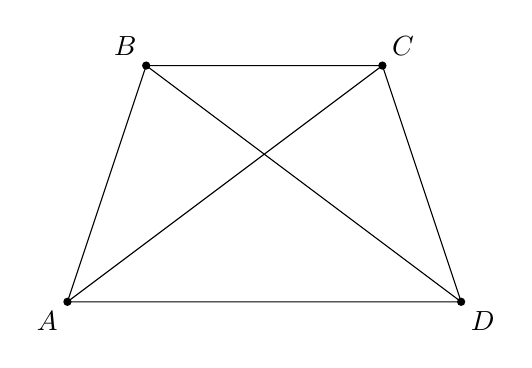
\begin{tikzpicture}[line join =round] 
		\coordinate (A) at (0,0);
		\coordinate (B) at (1,3);
		\coordinate (C) at (4,3);
		\coordinate (D) at (5,0);
		\draw (A)--(B)--(C)--(D)--cycle (D)--(B) (A)--(C);
		\fill (C) node[above right] {$C$} circle (1.5pt);
		\fill (B) node[above left] {$B$} circle (1.5pt);
		\fill (A) node[below left] {$A$} circle (1.5pt);
		\fill (D) node[below right] {$D$} circle (1.5pt);
	\end{tikzpicture}
\end{center}
\loigiai{Hình thang cân $ ABCD $ có hai cạnh bên $ AB=CD $ và hai đường chéo $ BD=AC $. \\Do đó, $ AB+BD=CD+AC>AD $.\\ Vậy 2 điểm $ B, C $ cùng thuộc một elip có hai tiêu điểm là $ A $ và $ D. $ }
\end{bt}

% nguồn: TuLuan_Lop10_Dot2 (nhập 14/11/2026)
\begin{bt}%[0H9V3-3] % KIEM_TRA%[Trường Nguyễn Minh Khai][Dự án đề kiểm tra HKII NH22-23-Nguyễn Tài Tuệ]%[ma:85031538]
  Trong mặt phẳng $Oxy$, cho đường thẳng $(\Delta)\colon x-2 y+2023=0$ và hai điểm $P(2; 5)$, $Q(5; 1)$.
\begin{enumerate}
	\item Viết phương trình đường thẳng $\left(d_1\right)$ đi qua điểm $P$ và song song với đường thẳng $(\Delta)$.
	\item Viết phương trình đường thẳng $\left(d_2\right)$ đi qua điểm $P$ và cách điểm $Q$ một khoảng bằng $  3  $.
\end{enumerate}  
   \loigiai{
   	\begin{enumerate}
   		\item Đường thẳng $ (d_1) $ song song với đường thẳng $ (\Delta) $ nên đường thẳng $ (d_1) $ có dạng $ x-2y+c=0 $, với $ c\ne 2023 $.\\
   		Mà $ P\in (d_1) $ nên $2-2\cdot 5+c=0 \Leftrightarrow c=8$.\\
   		Vậy phương trình đường thẳng $ d_1\colon x-2y+8=0 $.
   		\item Gọi $ \vec{n}(a;b) $ là một véc-tơ pháp tuyến của đường thẳng $ d_2 $, với $ a^2+b^2\ne 0 $.\\
   		Phương trình đường thẳng $ d_2 $ có dạng $ a(x-2)+b(y-5)=0 \Leftrightarrow ax+by-2a-5b=0$.\\
   		Ta có
   		\begin{eqnarray*}
   			&& \mathrm{d}(Q,(d_2)) =3\\
   			&\Leftrightarrow& \dfrac{|5a+b-2a-5b|}{\sqrt{a^2+b^2}}=3\\
   			&\Leftrightarrow& |3a-4b|=3\sqrt{a^2+b^2} \\
   			&\Leftrightarrow& 9a^2 -24ab+16b^2 =9(a^2+b^2) \\
   			&\Leftrightarrow& 7b^2-24ab =0\\
   			&\Leftrightarrow& \hoac{&b=0\\&7b-24a=0.}
   		\end{eqnarray*}  
   		\begin{itemize}
   			\item Với $b=0$, chọn $a=1$, suy ra phương trình đường thẳng $d_2\colon x-2=0$.
   			\item Với $ 7b-24a=0 $, chọn $ a=7, b=24 $, suy ra phương trình đường thẳng $$ d_2\colon 7x+24y-134=0.$$
   		\end{itemize}
   	\end{enumerate}
   }
\end{bt}

% nguồn: TuLuan_Lop10_Dot2 (nhập 14/11/2026)
\begin{bt}%[0H9H3-3]%[Dự án đề kiểm tra Giữa HKII NH22-23- Thành Lê]%[THPT Nguyễn Công Trứ]%[ma:516685ae]
	Xét vị trí tương đối của các cặp đường thẳng sau
	\begin{enumerate}
		\item $d_1\colon x + y - 3=0$; $d_2\colon 2x + 2y=0$
		\item $d_1\colon - 4x + 6y - 2=0$; $d_2\colon 2x - 3y + 1=0$.
	\end{enumerate}
	\loigiai{
	\begin{enumerate}
		\item
		\begin{itemize}
			\item $d_1$ và $d_2$ có  véc-tơ pháp tuyến lần lượt là $\vec{n_1}=(1;1)$ và $\vec{n_2}=(2;2)$.
			\item Ta có $\dfrac{1}{1}=\dfrac{2}{2}$, suy ra $\vec{n_1}$ và $\vec{n_2}$ cùng phương.
			\item  Lấy $M(1{,}2)\in d_1$, thay tọa độ $M$ vào $d_2$, ta được $2\cdot1+2\cdot2=6\neq0$, suy ra $M\not\in d_2$.
		\end{itemize}
		Vậy $d_1\parallel d_2$.
		\item 
		\begin{itemize}
			\item $d_1$ và $d_2$ có  véc-tơ pháp tuyến lần lượt là $\vec{n_1}=(-4;6)$ và $\vec{n_2}=(2;3)$.
			\item Ta có $\dfrac{-4}{6}\neq\dfrac{2}{3}$, suy ra $\vec{n_1}$ và $\vec{n_2}$ không cùng phương.
		\end{itemize}
		Vậy $d_1$ cắt $d_2$.
	\end{enumerate}
	}
\end{bt}

% nguồn: TuLuan_Lop10_Dot2 (nhập 14/11/2026)
\begin{bt}%[0H9H3-3]%[Dự án đề kiểm tra GHKII NH22-23- Phạm Phương]%[THPT Trường Chinh - Đề số A]%[ma:830298db]
	Trong mặt phẳng tọa độ $Oxy$, cho đường thẳng $d\colon x-7y+6=0$ và đường thẳng $\Delta\colon 3x+4y-5=0$.
	\begin{enumerate}
		\item Viết phương trình đường thẳng qua $M(-3;2)$ và song song đường thẳng $\Delta$.
		\item Tính góc giữa đường thẳng $\Delta$ và đường thẳng $d$.
	\end{enumerate}
	\loigiai{
	\begin{enumerate}
		\item Gọi đường thẳng cần tìm là $\Delta'$.
		\begin{itemize}
			\item $\Delta' \parallel \Delta$ nên $\Delta'$ có phương trình dạng $3x+4y+c=0$, $(c \neq -5)$.
			\item $\Delta'$ qua $M(-3;2)$ nên $3\cdot (-3)+4\cdot 2+c=0 \Leftrightarrow c=1$ (thoả mãn).
		\end{itemize}		
		Vậy $\Delta'\colon 3x+4y+1=0$.
		\item $\Delta$ và $d$ có véc-tơ pháp tuyến lần lượt là $\vec{n}_d=(1;-7)$, $\vec{n}_\Delta=(3;4)$. Gọi $\varphi$ là góc giữa đường thẳng $\Delta$ và đường thẳng $d$ ta có
		$$\cos \varphi = \dfrac{\left|\vec{n}_d\cdot \vec{n}_\Delta\right|}{\left|\vec{n}_d\right|\cdot \left|\vec{n}_\Delta\right|}=\dfrac{\left|1\cdot 3+(-7)\cdot 4\right|}{\sqrt{1^2+(-7)^2}\sqrt{3^2+4^2}}=\dfrac{\sqrt{2}}{2}.$$
		Vậy góc giữa đường thẳng $\Delta$ và đường thẳng $d$ là $\varphi = 45^\circ$.
	\end{enumerate}
}
\end{bt}

% nguồn: TuLuan_Lop10_Dot2 (nhập 14/11/2026)
\begin{bt}%[0H9H3-3]%[Tex hóa SGK CD-CT,T7/22, Lê Minh Thiện Anh]%[ma:331cb627]
	Cho đường thẳng $d$ có phương trình $4x+2y+1=0$. Xét vị trí tương đối của $d$ với mỗi đường thẳng sau:
	\begin{enumerate}
		\item $\Delta_1 \colon x-2y+4=0$;
		\item $\Delta_2 \colon 2x+y-9=0$;
		\item $\Delta_3 \colon \heva{&x=-\dfrac{1}{4}-t\\&y=2t.}$
	\end{enumerate}
	\loigiai{
		\begin{enumerate}
			\item $d$ và $\Delta_1$ có véc-tơ pháp tuyến lần lượt là $\overrightarrow{n}_1=(4;2)$ và $\overrightarrow{n}_2=(1;-2)$.\\
			Ta có: $a_1b_2-a_2b_1=4 \cdot (-2)-2 \cdot 1=-10 \ne 0$, suy ra $\overrightarrow{n}_1$ và $\overrightarrow{n}_2$ là hai véc-tơ không cùng phương. Vậy $d$ và $\Delta_1$ cắt nhau tại một điểm $M$.\\
			Giải hệ phương trình $\heva{&4x+2y+1=0\\&x-2y+4=0}$ ta được $M\left(-1;\dfrac{3}{2}\right)$.
			\item $d$ và $\Delta_2$ có véc-tơ pháp tuyến lần lượt là $\overrightarrow{n}_1=(4;2)$ và $\overrightarrow{n}_2=(2;1)$.\\
			Ta có $\dfrac{4}{2}=\dfrac{2}{1}$ suy ra $\overrightarrow{n}_1$ và $\overrightarrow{n}_2$ là hai véc-tơ cùng phương. Vậy $d$ và $\Delta_2$ song song hoặc trùng nhau. Lấy điểm $N\left(0;-\dfrac{1}{2}\right)$ thuộc $d$, thay tọa độ của $N$ vào phương trình $\Delta_2$, ta được $2 \cdot 0-\dfrac{1}{2}-9 \ne 0$, suy ra $N$ không thuộc $\Delta_2$. Vậy $d\parallel\Delta_2$.
			\item Ta có $\Delta_3 \colon \heva{&x=-\dfrac{1}{4}-t\\&y=2t.}$\\
			Suy ra: phương trình tổng quát của $\Delta_3 \colon 2x+y+\dfrac{1}{2}=0$.\\
			$d$ và $\Delta_3$ có véc-tơ pháp tuyến lần lượt là $\overrightarrow{n}_1=(4;2)$ và $\overrightarrow{n}_2=(2;1)$. Ta có $\dfrac{4}{2}=\dfrac{2}{1}$ suy ra $\overrightarrow{n}_1$ và $\overrightarrow{n}_2$ là hai véc-tơ cùng phương. Vậy $d$ và $\Delta_3$ song song hoặc trùng nhau.\\
			Lấy điểm $P\left(-\dfrac{1}{4};0\right)$ thuộc $d$, thay tọa độ của $P$ vào phương trình tổng quát của $\Delta_3$, ta được $2\left(-\dfrac{1}{4}\right)+0+\dfrac{1}{2}=0$, suy ra $N$ thuộc $\Delta_3$. Vậy $d\equiv\Delta_3$.
		\end{enumerate}
	}
\end{bt}

% nguồn: TuLuan_Lop10_Dot2 (nhập 14/11/2026)
\begin{bt}%[0H9H3-3]%[Tex hóa SGK CD-CT,T7/22, Lê Minh Thiện Anh]%[ma:7cd4f341]
	Xét vị trí tương đối của các cặp đường thẳng $d_1$ và $d_2$ sau đây:
	\begin{enumerate}
		\item $d_1 \colon 2x+y+9=0$ và $d_2 \colon 2x+3y-9=0$;
		\item $d_1 \colon \heva{&x=2+t\\&y=1-2t}$ và $d_2 \colon 2x+y+10=0$;
		\item $d_1 \colon \heva{&x=1-t\\&y=8-5t}$ và $d_2 \colon 5x-y+3=0$. 
	\end{enumerate}
	\loigiai{
		\begin{enumerate}
			\item $d_1$ và $d_2$ cắt nhau.\\
			$d_1$ và $d_2$ có véc-tơ pháp tuyến lần lượt là $\overrightarrow{n}_1=(2;1)$ và $\overrightarrow{n}_2=(2;3)$.\\
			Ta có: $a_1b_2-a_2b_1=2 \cdot 3-1 \cdot 2=4 \ne 0$, suy ra $\overrightarrow{n}_1$ và $\overrightarrow{n}_2$ là hai véc-tơ không cùng phương. Vậy $d_1$ và $d_2$ cắt nhau tại một điểm $M$.\\
			Giải hệ phương trình $\heva{&2x+y+9=0\\&2x+3y-9=0}$ ta được $M\left(-9;9\right)$.
			\item $d_1$ và $d_2$ song song.\\
			$d_1$ và $d_2$ có véc-tơ pháp tuyến lần lượt là $\overrightarrow{n}_1=(2;1)$ và $\overrightarrow{n}_2=(2;1)$.\\
			Ta có $\overrightarrow{n}_1$ và $\overrightarrow{n}_2$ là hai véc-tơ cùng phương. Vậy $d_1$ và $d_2$ song song hoặc trùng nhau. Lấy điểm $N\left(1;2\right)$ thuộc $d_1$, thay tọa độ của $N$ vào phương trình $d_2$, ta được $2 \cdot 2+1+10 \ne 0$, suy ra $N$ không thuộc $d_2$. Vậy $d_1\parallel d_2$.
			\item $d_1$ và $d_2$ trùng nhau.\\
			Ta có $d_1 \colon \heva{&x=1-t\\&y=8-5t.}$\\
			Suy ra: phương trình tổng quát của $d_1 \colon 5x-y+3=0$.\\
			Vậy $d_1\equiv d_2$.
		\end{enumerate}
	}
\end{bt}

% nguồn: TuLuan_Lop10_Dot2 (nhập 14/11/2026)
\begin{bt}%[0H9H3-3]%[0H3B1]%[ma:e419e43b]
	Cho hai đường thẳng $\Delta: (m+3)x+3y-2m+3=0$ và $\Delta': 2x+2y+2-3m=0$. Tìm giá trị của tham số $m$ để
	\begin{listEX}[1]
		\item Đường thẳng $\Delta$ cắt đường thẳng $\Delta'$.
		\item 	Đường thẳng $\Delta$ song song với $\Delta'$.
	\end{listEX}
	\loigiai{
	\begin{listEX}[1]
			\item
			$\Delta$ cắt $\Delta'$ khi và chỉ khi $\dfrac{m+3}{2}\neq \dfrac{3}{2}\Leftrightarrow m\neq 0$.\\
			\item	Theo câu a), để $\Delta$ song song với $\Delta'$ thì trước hết ta phải có $m=0$.\\
			Với $m=0$, khi đó dễ dàng nhận thấy $\Delta \equiv \Delta'$.\\
			Vậy không tồn tại $m$ để $\Delta \parallel \Delta'$.
		\end{listEX}
		\emph{Chú ý}: Ta có thể làm theo cách sau: $\Delta$ song song với $\Delta'$ khi và chỉ khi $$\heva{\dfrac{m+3}{2}&=\dfrac{3}{2}\neq\dfrac{-2m+3}{2-3m}\\2-3m&\neq0}$$
		Hệ trên vô nghiệm, do đó không tồn tại $m$ để $\Delta \parallel \Delta'$.\\
	}
\end{bt}

% nguồn: TuLuan_Lop10_Dot2 (nhập 14/11/2026)
\begin{bt}%[0H9H3-3]%[0H3K1]%[ma:d41b39b8]
	Cho các đường thẳng $\Delta: 2x+3y-5=0, \Delta': 3x-2y-1=0$ và điểm $M(2;3)$. 
	\begin{listEX}[1]
	\item Xét vị trí tương đối giữa các đường thẳng $\Delta$ và $\Delta'$.
	\item Biết $d$ là đường thẳng đi qua điểm $M$ và tạo với các đường thẳng $\Delta,\Delta'$ một tam giác cân. Tính góc giữa các đường thẳng $\Delta$ và $d$.
	\end{listEX}
	\loigiai{
	\begin{listEX}[1]
	\item Ta có $\overrightarrow{n}=(2{,}3)$ và $\overrightarrow{n'}=(3,-2)$ là các véc-tơ pháp tuyến của $\Delta$ và $\Delta'$.\\
		Ta thấy $\overrightarrow{n}$ và $\overrightarrow{n'}$ không cùng phương vì $\dfrac{2}{3}\neq \dfrac{3}{-2}$, từ đó suy ra $\Delta$ và $\Delta'$ là các đường thẳng cắt nhau.
	\item Ta có  $\overrightarrow{n}.\overrightarrow{n'}=2.3+3.(-2)=0$, do đó $\Delta$ và $\Delta'$ là các đường thẳng vuông góc với nhau.\\
		Gọi $A=\Delta\cap\Delta'$, $B=\Delta\cap d$, $C=d\cap\Delta'$. Khi đó tam giác $ABC$ là vuông tại $A$ do đó nếu tam giác $ABC$ cân thì $\widehat{B}=\widehat{C}=\dfrac{\pi}{4}$.\\
		Từ đó suy ra góc giữa các đường thẳng $\Delta$ và $d$ bằng $\dfrac{\pi}{4}$.
	\end{listEX}
}
\end{bt}

% nguồn: TuLuan_Lop10_Dot2 (nhập 14/11/2026)
\begin{bt}%[0H9H3-3]%[ma:b11cd2f2]
	Trong mặt phẳng tọa độ $Oxy$, cho ba đường thẳng $d_1$: $2x+y-4=0$, $d_2$: $5x-2y+3=0$, $d_3$: $mx+3y-2=0$.\
	\begin{listEX}[1]
		\item Xét vị trí tương đối giữa $d_1$ và $d_2$.
		\item Tìm giá trị của tham số $m$ để 3 đường thẳng trên đồng quy.
	\end{listEX}
	\loigiai{
	\begin{listEX}[1]
			\item Nhận thấy $\dfrac{2}{5}\neq \dfrac{1}{-2}$, từ đó suy ra các đường thẳng $d_1$, $d_2$ cắt nhau.
			\item Tọa độ giao điểm của hai đường thẳng $d_1$ và $d_2$ là nghiệm của hệ phương trình: $$\heva{2x+y-4&=0\\5x-2y+3&=0}\Leftrightarrow\heva{x&=\dfrac{5}{9}\\y&=\dfrac{26}{9}}.$$
			Vậy $d_1$ và $d_2$ cắt nhau tại điểm $M\left(\dfrac{5}{9};\dfrac{26}{9}\right)$.\\
			Vì $d_1$, $d_2$, $d_3$ đồng quy nên $M\in d_3$, ta có: $m.\dfrac{5}{9}+3.\dfrac{26}{9}-2=0$ $\Leftrightarrow$ $m=-12$
	\end{listEX}
	}
\end{bt}

% nguồn: TuLuan_Lop10_Dot2 (nhập 14/11/2026)
\begin{bt}%[0H9H3-3]%[ma:a6cb846b]
	Trong mặt phẳng với hệ trục tọa độ $Oxy$ cho các đường thẳng $\Delta\colon3x +5y + 15=0$ và $\Delta'\colon\heva{& x=10 - 3t\\& y=1 + 5t}$. Tính góc $\varphi$ giữa $\Delta$ và $\Delta'$.
	\loigiai{
		Ta có $\overrightarrow{n}=(3;5)$ là một véc-tơ pháp tuyến của $\Delta$.\\
		$\overrightarrow{u'}=(-3;5)$ là một véc-tơ chỉ phương của $\Delta'$, suy ra $\Delta'$ có véc-tơ pháp tuyến $\overrightarrow{n'}=(5;3).$\\
		Do $\overrightarrow{n}\cdot\overrightarrow{n'}=0 \Rightarrow \Delta\bot \Delta'.$\\
		Vậy $\varphi=90^\circ$ 
	}
\end{bt}

% nguồn: TuLuan_Lop10_Dot2 (nhập 14/11/2026)
\begin{bt}%[0H9V3-3]%[0H3G2]%[ma:a54908c2]
	Trong hệ trục tọa độ $Oxy$, cho hai đường thẳng $d_1\colon 2x+my=2m$ và $d_2\colon 2mx-y+2=0$. Đường thẳng $d_1$ cắt tia $Ox$ tại $A$, đường thẳng $d_2$ cắt trục $Ox$ tại $B$ và hai đường thẳng $d_1$, $d_2$ cắt nhau tại $C$. Tìm $m$ để diện tích tam giác $ABC$ đạt giá trị nhỏ nhất.
	\loigiai{
		Ta có $d_1$ cắt $Ox$ tại $A(m;0)$, $d_2$ cắt $Ox$ tại $B\left(-\dfrac{1}{m};0\right)$, $m\ne 0$.\\
		Hai đường thẳng $d_1$, $d_2$ cắt nhau tại $C$ nên tọa độ $C$ thỏa hệ
		$$\heva{&2x+my=2m\\&2mx-y+2=0}\Leftrightarrow \heva{&2x+my=2m\\&2m^2x-my=-2m}\Leftrightarrow \heva{&2x+my=2m\\&2(m^2+1)x=0}\Leftrightarrow \heva{&x=0\\&y=2}\Rightarrow C(0;2).$$
		Khi đó
		\begin{eqnarray*}
			S_{\triangle ABC}&=&\dfrac{1}{2}\cdot \mathrm{d}(C,AB)\cdot AB\\
			&=&\dfrac{1}{2}\cdot 2\cdot \left|\dfrac{1}{m}+m\right|\\
			&=&\left|\dfrac{1}{m}\right|+|m|\text{ do }\dfrac{1}{m}\cdot m\ge0\\
			&\ge& 2\sqrt{\left|\dfrac{1}{m}\right|\cdot |m|}\\
			&=& 2.
		\end{eqnarray*}
		Dấu ``$=$'' xảy ra khi $\left|\dfrac{1}{m}\right|=|m|\Leftrightarrow m=\pm 1$.
	}
\end{bt}

% nguồn: TuLuan_Lop10_Dot2 (nhập 14/11/2026)
\begin{bt}%[0H9V3-3]%[ma:777a847c]
	Trong mỗi trường hợp sau, tìm các giá trị của tham số $m$ sao cho ba đường thẳng sau đây phân biệt và đồng quy.
	\begin{enumEX}{1}
		\item $d_1\colon y=2x$; $d_2\colon y=-x-3$; $d_3\colon y=mx+5$.
		\item $d_1\colon y=2x-1$; $d_2\colon y=8-x$; $d_3\colon y=(3-2m)x+2$.
	\end{enumEX}
	\loigiai{
		\begin{enumEX}{1}
			\item Gọi $A=d_1\cap d_2 \Rightarrow A(-1;-2)$.\\
			Để ba đường thẳng đã cho đồng quy thì $\heva{& m\neq2\\& m\neq-1\\& A(-1;-2)\in d_3} \Leftrightarrow \heva{& m\neq2\\& m\neq-1\\& -m+5=-2} \Leftrightarrow \heva{& m\neq2\\& m\neq-1\\& m=7 \quad\text{(nhận)}.}$
			\item Gọi $A=d_1\cap d_2 \Rightarrow A(3;3)$.\\
			Để ba đường thẳng đã cho đồng quy thì $\heva{& 3-2m\neq2\\& 3-2m\neq-1\\& A(3;3)\in d_3} \Leftrightarrow \heva{& m\neq\dfrac{1}{2}\\& m\neq2\\& 3(3-2m)+2=3} \Leftrightarrow \heva{& m\neq\dfrac{1}{2}\\& m\neq2\\& m=\dfrac{4}{3} \quad\text{(nhận)}.}$
		\end{enumEX}
	}
\end{bt}

% nguồn: TuLuan_Lop10_Dot2 (nhập 14/11/2026)
\begin{bt}%[0H9H3-3]%[Tex hóa SGK CD,T8/22, Phạm Doãn Lê Bình]%[ma:88875092]
	Xét vị trí tương đối của mỗi cặp đường thẳng sau
	\begin{enumerate}
		\item $\Delta_1\colon 2x-y+1=0$ và $\Delta_2\colon -x+2y+2=0$.
		\item $\Delta_3\colon x-y-1=0$ và $\Delta_4\colon \heva{& x = 1 + 2t \\ & y = 3+2t.}$
	\end{enumerate}
	\loigiai{
		\begin{enumerate}
			\item Đường thẳng $\Delta_1$ có véc-tơ chỉ phương $\vec{u}_1=(1;2)$, đường thẳng $\Delta_2$ có véc-tơ chỉ phương $\vec{u}_2=(-2;-1)$.\\
			Do $\dfrac{1}{-2}\ne \dfrac{2}{-1}$ nên $\vec{u}_1$, $\vec{u}_2$ không cùng phương, suy ra $\Delta_1$ cắt $\Delta_2$.
			\item Đường thẳng $\Delta_3$, $\Delta_4$ lần lượt có véc-tơ chỉ phương $\vec{u}_3=(1 ; 1)$, $\vec{u}_4=(2 ; 2)$. Suy ra $\vec{u}_4=2 \vec{u}_3$. \\
			Chọn $t=0$, ta có điểm $M(1 ; 3) \in \Delta_4$. Do $1-3-1 \neq 0$ nên $M(1 ; 3) \notin \Delta_3$. Vậy $\Delta_3$ song song với $\Delta_4$.
		\end{enumerate}
	}
\end{bt}

% nguồn: TuLuan_Lop10_Dot2 (nhập 14/11/2026)
\begin{bt}%[0H9H3-3]%[Tex hóa SGK CD,T8/22, Phạm Doãn Lê Bình]%[ma:1188a8af]
	Xét vị trí tương đối của hai đường thẳng \[\Delta_1\colon \heva{& x=1+t_1 \\ & y = -2+t_1} \text{ và } \Delta_2\colon \heva{& x = 2t_2 \\ & y = -3+2t_2.}\]
	\loigiai{
		Đường thẳng $\Delta_1$ có một véc-tơ chỉ phương $\vec{u}_1=(1;1)$.\\
		Đường thẳng $\Delta_2$ có một véc-tơ chỉ phương $\vec{u}_2=(2;2)$.\\
		Ta có $\vec{u}_2=2\vec{u}_1$ nên $\vec{u}_1$, $\vec{u}_2$ cùng phương. Suy ra $\Delta_1$ song song hoặc trùng với $\Delta_2$.\\
		Cho $t_1=0$ ta có điểm $A(1;-2)$ thuộc đường thẳng $\Delta_1$.\\
		Thay $x=1$, $y=-2$ vào phương trình đường thẳng $\Delta_2$ ta có
		\[ \heva{& 1 = 2t_2 \\ & -2=-3+2t_2} \Leftrightarrow \heva{& t_2=\dfrac{1}{2}\\ & t_2=\dfrac{1}{2}} \Leftrightarrow t_2=\dfrac{1}{2}.\]
		Vậy $A\in\Delta_2$. Suy ra $\Delta_1$ và $\Delta_2$ trùng nhau.
	}
\end{bt}

% nguồn: TuLuan_Lop10_Dot2 (nhập 14/11/2026)
\begin{bt}%[0H9H3-3]%[Tex hóa SGK CD,T8/22, Phạm Doãn Lê Bình]%[ma:e0e98aa5]
	Xét vị trí tương đối của hai đường thẳng $\Delta_1\colon x-2 y+1=0$ và $\Delta_2\colon 2 x-4 y+2=0$.
	\loigiai{
		Tọa độ giao điểm của đường thẳng $\Delta_1$ và đường thẳng $\Delta_2$ là nghiệm của hệ phương trình
		\[\heva{& x-2 y+1=0 \\ & 2 x-4 y+2=0.}\]
		Hệ trên có vô số nghiệm.\\
		Như vậy, $\Delta_1$ và $\Delta_2$ có vô số điểm chung, tức là $\Delta_1$ trùng với $\Delta_2$.
	}
\end{bt}

% nguồn: TuLuan_Lop10_Dot2 (nhập 14/11/2026)
\begin{bt}%[0H9H3-3]%[Tex hóa SGK CD,T8/22, Phạm Doãn Lê Bình]%[ma:43ab3af4]
	Xét vị trí tương đối củađường thẳng $d\colon x+2y-2=0$ với mỗi đường thẳng sau\\
	$\Delta_1\colon 3x-2y+6=0$;\\
	$\Delta_2\colon x+2y+2=0$;\\
	$\Delta_3\colon 2x+4y-4=0$.
	\loigiai{
		\begin{itemize}
			\item[$\bullet$] Tọa độ giao điểm của đường thẳng $d$ và đường thẳng $\Delta_1$ là nghiệm của hệ phương trình
			\[\heva{& x+2 y-2=0 \\ & 3 x-2 y+6=0.}\]
			Hệ trên có nghiệm duy nhất nên $d$ và $\Delta_1$ có một điểm chung duy nhất, tức là $d$ cắt $\Delta_1$.
			\item[$\bullet$] Tọa độ giao điểm của đường thẳng $d$ và đường thẳng $\Delta_2$ là nghiệm của hệ phương trình
			\[\heva{& x+2 y-2=0 \\ &  x+2 y+2=0.}\]
			Hệ trên vô nghiệm nên $d$ và $\Delta_2$ không có điểm chung, tức là $d$ song song với $\Delta_2$.
			\item[$\bullet$] Tọa độ giao điểm của đường thẳng $d$ và đường thẳng $\Delta_2$ là nghiệm của hệ phương trình
			\[\heva{& x+2 y-2=0 \\ &  2x+4 y-4=0.}\]
			Hệ trên có vô số nghiệm nên $d$ và $\Delta_3$ có vô số điểm chung, tức là $d$ trùng với $\Delta_3$.
		\end{itemize}
	}
\end{bt}

% nguồn: TuLuan_Lop10_Dot2 (nhập 14/11/2026)
\begin{bt}%[0H9H3-3]%[Hoàng Thanh Phương - ĐGNL-ĐGTD-2022]%[ma:029ef2c8]
	Cho hai đường thẳng $\Delta\colon (m+3)x+3y-2m+3=0$ và $\Delta'\colon 2x+2y+2-3m=0$. Tìm giá trị của tham số $m$ để
	\begin{enumerate}[a)]
		\item Hai đường thẳng song song.
		\item Hai đường thẳng cắt nhau.
	\end{enumerate}
\loigiai{
\begin{enumerate}[a)]
	\item Hai đường thẳng $\Delta$ và $\Delta'$ song song khi và chỉ khi
	$$\dfrac{m+3}{2}=\dfrac{3}{2}\neq\dfrac{-2m+3}{2-3m}$$
	Vì $\dfrac{m+3}{2}=\dfrac{3}{2}\Leftrightarrow m=0$, mà thay $m=0$ vào phương trình $\Delta$ và $\Delta'$ thì ta thấy $\Delta\equiv\Delta'$ nên không tồn tại giá trị của tham số $m$ để hai đường thẳng song song
	\item Hai đường thẳng $\Delta$ và $\Delta'$ cắt nhau khi và chỉ khi
	$$\dfrac{m+3}{2}\neq\dfrac{3}{2}\Leftrightarrow m\neq 0.$$
	Vậy với $m\neq 0$ thì $\Delta$ cắt $\Delta'$.
\end{enumerate}
}
\end{bt}
